\documentclass[a4paper,12pt]{article}

% ----- Packages ----------------------------------------------------------------------------------
\usepackage{array}
\usepackage[capposition=top]{floatrow}
  \floatsetup[table]{font=small}
\usepackage{geometry}
  \geometry{verbose,tmargin=2cm,bmargin=2.5cm,lmargin=2cm,rmargin=2.25cm,footskip=1.5cm}
\usepackage[bookmarks, hidelinks]{hyperref}
\usepackage{multirow}
\usepackage{setspace}
  \onehalfspacing
\usepackage[font=small]{caption}
\usepackage[font=small]{subcaption}
\usepackage[textsize=normalsize]{todonotes}

% Set paths
\makeatletter
\graphicspath{{graphs/}}
\def\input@path{{tables/}}
\makeatother

% -------------------------------------------------------------------------------------------------

% ----- Opening -----------------------------------------------------------------------------------
\title{Does the Added Worker Effect Matter? \\
Figures and Tables
}

\author{Nezih Guner\footnote{
  CEMFI.
  Email: \href{mailto://nezih.guner@cemfi.es}{nezih.guner@cemfi.es}.
  }
\and Yuliya A. Kulikova\footnote{
  Okinawa Institute of Science and Technology and International Institute for Applied Systems Analysis
  Email: \href{mailto://yuliya.kulikova@gmail.com}{yuliya.kulikova@gmail.com}.
  }
\and Arnau Valladares-Esteban\footnote{
  University of St. Gallen and SEW.
  Email: \href{mailto://arnau.valladares@gmail.com}{arnau.valladares@gmail.com}.
  }
}
\date{}

% Start document
\begin{document}
\maketitle
\newpage
%==================================================================================================
%----- BEGIN TABLE -----
\begin{table}[H]
  \centering
	\caption{The Added Worker Effect, Married Women}
  \def\arraystretch{1.25}
  \resizebox{\textwidth}{!}{
\begin{tabular}{l|c|c|c|c|c|c|c|c|c}
\hline
\hline
& 1976 & & & 1976 & 1980 & 1990 & 2000 & 2010 & 2020 \\
& to & Expansions & Recessions & to & to & to & to & to & to \\
& 2019 & & & 1979 & 1989 & 1999 & 2009 & 2019 & 2021 \\
\hline
\noalign{\smallskip}
\multicolumn{10}{l}{\textbf{Contemporaneous Effect}} \\
\noalign{\smallskip}
\hline
N to P
& 5.967 & 6.082 & 5.483 & 6.521 & 4.746 & 5.501 & 6.105 & 7.532 & 3.721 \\
& {\scriptsize (5.361, 6.573)}
& {\scriptsize (5.417, 6.746)}
& {\scriptsize (4.022, 6.945)}
& {\scriptsize (4.748, 8.294)}
& {\scriptsize (3.803, 5.689)}
& {\scriptsize (4.150, 6.851)}
& {\scriptsize (4.731, 7.479)}
& {\scriptsize (5.982, 9.081)}
& {\scriptsize (0.286, 7.157)}
\\ [0.1cm]
\hline
N to E
& 0.516 & 0.645 & -0.019 & 0.495 & -0.191 & 0.223 & 0.351 & 2.032 & -0.458 \\
& {\scriptsize (0.063, 0.970)}
& {\scriptsize (0.144, 1.146)}
& {\scriptsize (-1.057, 1.019)}
& {\scriptsize (-0.735, 1.726)}
& {\scriptsize (-0.844, 0.462)}
& {\scriptsize (-0.798, 1.243)}
& {\scriptsize (-0.703, 1.404)}
& {\scriptsize (0.803, 3.261)}
& {\scriptsize (-3.145, 2.230)}
\\ [0.1cm]
\hline
N to U
& 5.450 & 5.437 & 5.502 & 6.026 & 4.937 & 5.278 & 5.754 & 5.499 & 4.179 \\
& {\scriptsize (4.959, 5.941)}
& {\scriptsize (4.901, 5.972)}
& {\scriptsize (4.279, 6.725)}
& {\scriptsize (4.555, 7.496)}
& {\scriptsize (4.169, 5.704)}
& {\scriptsize (4.200, 6.357)}
& {\scriptsize (4.611, 6.898)}
& {\scriptsize (4.240, 6.758)}
& {\scriptsize (1.385, 6.974)}
\\ [0.1cm]
\hline
\noalign{\smallskip}
\multicolumn{10}{l}{\textbf{Effect with Leads and Lags}} \\
\noalign{\smallskip}
\hline
N to P
& 3.643 & 3.767 & 3.142 & 3.463 & 2.980 & 3.613 & 3.394 & 4.556 & 2.402 \\
& {\scriptsize (3.219, 4.067)}
& {\scriptsize (3.301, 4.234)}
& {\scriptsize (2.132, 4.151)}
& {\scriptsize (2.230, 4.696)}
& {\scriptsize (2.306, 3.654)}
& {\scriptsize (2.658, 4.569)}
& {\scriptsize (2.451, 4.338)}
& {\scriptsize (3.475, 5.637)}
& {\scriptsize (-0.096, 4.901)}
\\ [0.1cm]
\hline
N to E
& -0.124 & -0.071 & -0.196 & -0.358 & -0.406 & -0.200 & -0.382 & 0.635 & -0.262 \\
& {\scriptsize (-0.448, 0.199)}
& {\scriptsize (-0.428, 0.286)}
& {\scriptsize (-0.951, 0.558)}
& {\scriptsize (-1.242, 0.525)}
& {\scriptsize (-0.895, 0.084)}
& {\scriptsize (-0.939, 0.538)}
& {\scriptsize (-1.120, 0.355)}
& {\scriptsize (-0.212, 1.481)}
& {\scriptsize (-2.292, 1.769)}
\\ [0.1cm]
\hline
N to U
& 3.767 & 3.838 & 3.338 & 3.821 & 3.386 & 3.814 & 3.777 & 3.921 & 2.664 \\
& {\scriptsize (3.438, 4.096)}
& {\scriptsize (3.477, 4.200)}
& {\scriptsize (2.548, 4.128)}
& {\scriptsize (2.851, 4.791)}
& {\scriptsize (2.866, 3.906)}
& {\scriptsize (3.084, 4.544)}
& {\scriptsize (3.034, 4.520)}
& {\scriptsize (3.068, 4.774)}
& {\scriptsize (0.755, 4.572)}
\\ [0.1cm]
\hline
\hline
\end{tabular}
}


	\floatfoot{\textbf{Notes}:
    CPS 1976 to 2021.
    Each cell reports the estimated coefficient $\alpha$, expressed in percentage points, from Equation~1.
    We include all spouses who move from employment to unemployment.
    We report 95\% confidence intervals.
    We use dummies to non-parametrically control for each category of age, education, race, occupation, industry, and own children in the household of both spouses.
  }
\end{table}
%----- END TABLE ----

%----- BEGIN TABLE -----
\begin{table}[H]
  \centering
	\caption{The Added Worker Effect, Married Men}
  \def\arraystretch{1.25}
  \resizebox{\textwidth}{!}{
\begin{tabular}{l|c|c|c|c|c|c|c|c|c}
\hline
\hline
& 1976 & & & 1976 & 1980 & 1990 & 2000 & 2010 & 2020 \\
& to & Expansions & Recessions & to & to & to & to & to & to \\
& 2019 & & & 1979 & 1989 & 1999 & 2009 & 2019 & 2021 \\
\hline
\noalign{\smallskip}
\multicolumn{10}{l}{\textbf{Contemporaneous Effect}} \\
\noalign{\smallskip}
\hline
N to P
& 6.693 & 6.825 & 5.488 & 5.082 & 5.427 & 7.235 & 7.038 & 6.677 & 0.180 \\
& {\scriptsize (4.668, 8.719)}
& {\scriptsize (4.690, 8.961)}
& {\scriptsize (-0.770, 11.746)}
& {\scriptsize (-2.315, 12.478)}
& {\scriptsize (0.920, 9.934)}
& {\scriptsize (2.924, 11.547)}
& {\scriptsize (3.130, 10.946)}
& {\scriptsize (2.771, 10.583)}
& {\scriptsize (-9.322, 9.681)}
\\ [0.1cm]
\hline
N to E
& 0.874 & 0.793 & 1.989 & -3.706 & -1.037 & 0.354 & 1.574 & 2.412 & 1.456 \\
& {\scriptsize (-0.780, 2.528)}
& {\scriptsize (-0.940, 2.525)}
& {\scriptsize (-3.353, 7.331)}
& {\scriptsize (-8.016, 0.603)}
& {\scriptsize (-4.259, 2.184)}
& {\scriptsize (-2.865, 3.572)}
& {\scriptsize (-1.786, 4.935)}
& {\scriptsize (-0.975, 5.800)}
& {\scriptsize (-8.377, 11.290)}
\\ [0.1cm]
\hline
N to U
& 5.819 & 6.033 & 3.499 & 8.788 & 6.464 & 6.882 & 5.464 & 4.265 & -1.277 \\
& {\scriptsize (4.122, 7.517)}
& {\scriptsize (4.224, 7.842)}
& {\scriptsize (-1.275, 8.272)}
& {\scriptsize (1.615, 15.961)}
& {\scriptsize (2.626, 10.302)}
& {\scriptsize (3.062, 10.702)}
& {\scriptsize (2.230, 8.698)}
& {\scriptsize (1.173, 7.356)}
& {\scriptsize (-8.107, 5.554)}
\\ [0.1cm]
\hline
\noalign{\smallskip}
\multicolumn{10}{l}{\textbf{Effect with Leads and Lags}} \\
\noalign{\smallskip}
\hline
N to P
& 3.851 & 4.075 & 1.867 & 5.472 & 3.596 & 4.796 & 3.914 & 3.001 & 1.971 \\
& {\scriptsize (2.359, 5.342)}
& {\scriptsize (2.495, 5.655)}
& {\scriptsize (-2.613, 6.348)}
& {\scriptsize (-0.548, 11.492)}
& {\scriptsize (0.199, 6.992)}
& {\scriptsize (1.584, 8.007)}
& {\scriptsize (1.090, 6.738)}
& {\scriptsize (0.115, 5.886)}
& {\scriptsize (-5.205, 9.148)}
\\ [0.1cm]
\hline
N to E
& -0.429 & -0.384 & -0.299 & -3.405 & -1.728 & 0.205 & 0.076 & -0.003 & 0.153 \\
& {\scriptsize (-1.631, 0.774)}
& {\scriptsize (-1.655, 0.887)}
& {\scriptsize (-3.938, 3.339)}
& {\scriptsize (-6.860, 0.050)}
& {\scriptsize (-4.181, 0.726)}
& {\scriptsize (-2.355, 2.766)}
& {\scriptsize (-2.314, 2.466)}
& {\scriptsize (-2.393, 2.387)}
& {\scriptsize (-6.520, 6.825)}
\\ [0.1cm]
\hline
N to U
& 4.280 & 4.459 & 2.167 & 8.877 & 5.323 & 4.590 & 3.838 & 3.004 & 1.819 \\
& {\scriptsize (3.070, 5.490)}
& {\scriptsize (3.169, 5.749)}
& {\scriptsize (-1.298, 5.631)}
& {\scriptsize (3.158, 14.595)}
& {\scriptsize (2.472, 8.175)}
& {\scriptsize (1.950, 7.231)}
& {\scriptsize (1.575, 6.102)}
& {\scriptsize (0.737, 5.271)}
& {\scriptsize (-4.098, 7.735)}
\\ [0.1cm]
\hline
\hline
\end{tabular}
}

	\floatfoot{\textbf{Notes}:
    CPS 1976 to 2021.
    Each cell reports the estimated coefficient $\alpha$, expressed in percentage points, from Equation~1.
    We include all spouses who move from employment to unemployment.
    We report 95\% confidence intervals.
    We use dummies to non-parametrically control for each category of age, education, race, occupation, industry, and own children in the household of both spouses.
  }
\end{table}
%----- END TABLE ----

%----- BEGIN TABLE -----
\begin{table}[H]
  \centering
	\caption{Shares of Added Workers, Married Women}
  \def\arraystretch{1.25}
  \resizebox{\textwidth}{!}{
\begin{tabular}{c|c|c|c|c|c|c|c|c}
\hline
\hline
1976 & & & 1976 & 1980 & 1990 & 2000 & 2010 & 2020 \\
to & Expansions & Recessions & to & to & to & to & to & to \\
2019 & & & 1979 & 1989 & 1999 & 2009 & 2019 & 2021 \\
\hline
\noalign{\smallskip}
\multicolumn{9}{l}{\textbf{Share of Non-participants among Married}} \\
\noalign{\smallskip}
\hline

29.731 &29.550 &31.266 &45.049 &34.470 &25.850 &26.181 &26.940 &26.076\\
{\scriptsize (29.704, 29.788)}
 &{\scriptsize (29.535, 29.618)}
 &{\scriptsize (31.143, 31.453)}
 &{\scriptsize (44.931, 45.383)}
 &{\scriptsize (34.338, 34.619)}
 &{\scriptsize (25.740, 25.979)}
 &{\scriptsize (26.133, 26.289)}
 &{\scriptsize (26.839, 26.967)}
 &{\scriptsize (25.851, 26.537)}
\\ [0.1cm]
\hline
\noalign{\smallskip}
\multicolumn{9}{l}{\textbf{Share of $ N$ to $ P$ among Non-participants}} \\
\noalign{\smallskip}
\hline

7.905 &7.903 &7.859 &6.743 &8.078 &8.593 &8.126 &7.234 &7.912\\
{\scriptsize (7.872, 7.972)}
 &{\scriptsize (7.873, 7.989)}
 &{\scriptsize (7.777, 8.029)}
 &{\scriptsize (6.667, 6.928)}
 &{\scriptsize (7.990, 8.166)}
 &{\scriptsize (8.513, 8.734)}
 &{\scriptsize (8.078, 8.295)}
 &{\scriptsize (7.138, 7.367)}
 &{\scriptsize (7.531, 8.114)}
\\ [0.1cm]
\hline
\noalign{\smallskip}
\multicolumn{9}{l}{\textbf{Share of Added Workers among $ N$ to $ P$}} \\
\noalign{\smallskip}
\hline

\noalign{\smallskip}
\multicolumn{9}{l}{Contemporaneous Effect} \\
\noalign{\smallskip}
\hline

1.456 &1.408 &1.907 &1.145 &1.651 &1.581 &1.401 &1.371 &1.825\\
{\scriptsize (1.422, 1.509)}
 &{\scriptsize (1.371, 1.441)}
 &{\scriptsize (1.718, 2.093)}
 &{\scriptsize (0.981, 1.284)}
 &{\scriptsize (1.533, 1.755)}
 &{\scriptsize (1.399, 1.669)}
 &{\scriptsize (1.168, 1.575)}
 &{\scriptsize (1.195, 1.544)}
 &{\scriptsize (1.109, 2.423)}
\\ [0.1cm]
\hline
\noalign{\smallskip}
\multicolumn{9}{l}{Effect with Leads and Lags} \\
\noalign{\smallskip}
\hline

3.494 &3.390 &4.384 &2.404 &3.913 &3.498 &3.354 &3.477 &5.053\\
{\scriptsize (3.432, 3.554)}
 &{\scriptsize (3.319, 3.451)}
 &{\scriptsize (4.027, 4.617)}
 &{\scriptsize (2.270, 2.536)}
 &{\scriptsize (3.806, 4.242)}
 &{\scriptsize (3.332, 3.771)}
 &{\scriptsize (3.014, 3.639)}
 &{\scriptsize (3.332, 3.895)}
 &{\scriptsize (4.044, 5.979)}
\\ [0.1cm]
\hline
\hline
\end{tabular}
}

	\floatfoot{\textbf{Notes}:
    CPS 1976 to 2021.
    Each cell reports a share in percentage.
    We include all spouses who move from employment to unemployment.
    We report 95\% confidence intervals from 1,000 bootstraps.
  }
\end{table}
%----- END TABLE ----

%----- BEGIN TABLE -----
\begin{table}[H]
  \centering
	\caption{Shares of Added Workers, Married Men}
  \def\arraystretch{1.25}
  \resizebox{\textwidth}{!}{
\begin{tabular}{c|c|c|c|c|c|c|c|c}
\hline
\hline
1976 & & & 1976 & 1980 & 1990 & 2000 & 2010 & 2020 \\
to & Expansions & Recessions & to & to & to & to & to & to \\
2019 & & & 1979 & 1989 & 1999 & 2009 & 2019 & 2021 \\
\hline
\noalign{\smallskip}
\multicolumn{9}{l}{\textbf{Share of Non-participants among Married}} \\
\noalign{\smallskip}
\hline

4.870 &4.908 &4.544 &3.665 &3.680 &4.581 &5.362 &6.269 &6.441\\
{\scriptsize (4.833, 4.902)}
 &{\scriptsize (4.870, 4.942)}
 &{\scriptsize (4.496, 4.597)}
 &{\scriptsize (3.576, 3.722)}
 &{\scriptsize (3.627, 3.727)}
 &{\scriptsize (4.514, 4.640)}
 &{\scriptsize (5.255, 5.417)}
 &{\scriptsize (6.209, 6.340)}
 &{\scriptsize (6.284, 6.589)}
\\ [0.1cm]
\hline
\noalign{\smallskip}
\multicolumn{9}{l}{\textbf{Share of $ N$ to $ P$ among Non-participants}} \\
\noalign{\smallskip}
\hline

14.625 &14.609 &14.731 &14.791 &15.896 &14.212 &14.307 &13.910 &16.419\\
{\scriptsize (14.421, 14.804)}
 &{\scriptsize (14.404, 14.782)}
 &{\scriptsize (14.430, 15.069)}
 &{\scriptsize (14.261, 15.107)}
 &{\scriptsize (15.733, 16.310)}
 &{\scriptsize (13.929, 14.614)}
 &{\scriptsize (14.116, 15.000)}
 &{\scriptsize (13.659, 14.102)}
 &{\scriptsize (16.066, 16.976)}
\\ [0.1cm]
\hline
\noalign{\smallskip}
\multicolumn{9}{l}{\textbf{Share of Added Workers among $ N$ to $ P$}} \\
\noalign{\smallskip}
\hline

\noalign{\smallskip}
\multicolumn{9}{l}{Contemporaneous Effect} \\
\noalign{\smallskip}
\hline

1.076 &1.057 &1.238 &1.398 &0.962 &1.143 &0.926 &1.195 &2.086\\
{\scriptsize (0.988, 1.175)}
 &{\scriptsize (0.982, 1.168)}
 &{\scriptsize (0.704, 1.394)}
 &{\scriptsize (0.795, 1.696)}
 &{\scriptsize (0.779, 1.218)}
 &{\scriptsize (0.961, 1.237)}
 &{\scriptsize (0.709, 1.226)}
 &{\scriptsize (0.857, 1.421)}
 &{\scriptsize (1.141, 2.481)}
\\ [0.1cm]
\hline
\noalign{\smallskip}
\multicolumn{9}{l}{Effect with Leads and Lags} \\
\noalign{\smallskip}
\hline

2.746 &2.657 &3.482 &2.376 &2.849 &2.857 &2.738 &2.751 &3.230\\
{\scriptsize (2.601, 2.945)}
 &{\scriptsize (2.546, 2.857)}
 &{\scriptsize (2.703, 3.957)}
 &{\scriptsize (1.935, 2.998)}
 &{\scriptsize (2.431, 3.116)}
 &{\scriptsize (2.601, 3.347)}
 &{\scriptsize (2.427, 2.923)}
 &{\scriptsize (2.440, 3.097)}
 &{\scriptsize (1.929, 3.609)}
\\ [0.1cm]
\hline
\hline
\end{tabular}
}

	\floatfoot{\textbf{Notes}:
    CPS 1976 to 2021.
    Each cell reports a share in percentage.
    We include all spouses who move from employment to unemployment.
    We report 95\% confidence intervals from 1,000 bootstraps.
  }
\end{table}
%----- END TABLE ----
%----- BEGIN TABLE -----
\begin{table}[H]
  \centering
  \caption{Transition Rates}
  \renewcommand{\arraystretch}{2}
  \begin{tabular}{c|c|c|c}
  \hline \hline
  $t-1$, $t$ & $E$ & $U$ & $N$ \\ \hline
  $E$        & $\frac{f_{EE}}{f_{EE}+f_{EU}+f_{EN}}$
             & $\frac{f_{EU}}{f_{EE}+f_{EU}+f_{EN}}$
             & $\frac{f_{EN}}{f_{EE}+f_{EU}+f_{EN}}$
             \\ \hline
  $U$        & $\frac{f_{UE}}{f_{UE}+f_{UU}+f_{UN}}$
             & $\frac{f_{UU}}{f_{UE}+f_{UU}+f_{UN}}$
             & $\frac{f_{UN}}{f_{UE}+f_{UU}+f_{UN}}$
             \\ \hline
  $N$        & $\frac{f_{NE}}{f_{NE}+f_{NU}+f_{NN}}$
             & $\frac{f_{NU}}{f_{NE}+f_{NU}+f_{NN}}$
             & $\frac{f_{NN}}{f_{NE}+f_{NU}+f_{NN}}$
             \\ \hline \hline
\end{tabular}

\end{table}
%----- END TABLE ----

%----- BEGIN FIGURE -----
\begin{figure}[H]
  \centering
  \caption{Individual Transition Probabilities, Married Women}
  \foreach \y in {E, U, N}{
    \foreach \t in {E, U, N}{
      \if \y\t
      \else
        \begin{subfigure}[b]{0.45\textwidth}
          \centering
          \includegraphics[scale= 0.125]{Y03_TQSA_Benchmark_\y to\t_DeNUN1_sex2.png}
          \caption{\y\ to \t}
        \end{subfigure}
      \fi
    }
  }
  \floatfoot{\textbf{Notes}:
    CPS 1976:Q1 to 2019:Q4.
    All values are in percent.
    We seasonally adjust monthly estimates using a 12-month moving average and report quarterly averages.
    The data is corrected for classification errors as described in Appendix~Section~A.1.
    Probabilities are corrected for time-aggregation bias as described in Appendix~Section~A.2.
    We report 95\% confidence intervals from 1,000 bootstraps.
    The vertical gray areas are NBER recession periods.
  }
\end{figure}
%----- END FIGURE -----
%
%----- BEGIN FIGURE -----
\begin{figure}[H]
  \centering
  \caption{Individual Transition Probabilities, Married Men}
  \foreach \y in {E, U, N}{
    \foreach \t in {E, U, N}{
      \if \y\t
      \else
        \begin{subfigure}[b]{0.45\textwidth}
          \centering
          \includegraphics[scale= 0.125]{Y03_TQSA_Benchmark_\y to\t_DeNUN1_sex1.png}
          \caption{\y\ to \t}
        \end{subfigure}
      \fi
    }
  }
  \floatfoot{\textbf{Notes}:
    CPS 1976:Q1 to 2019:Q4.
    All values are in percent.
    We seasonally adjust monthly estimates using a 12-month moving average and report quarterly averages.
    The data is corrected for classification errors as described in Appendix~Section~A.1.
    Probabilities are corrected for time-aggregation bias as described in Appendix~Section~A.2.
    We report 95\% confidence intervals from 1,000 bootstraps.
    The vertical gray areas are NBER recession periods.
  }
\end{figure}
%----- END FIGURE -----

%----- BEGIN FIGURE -----
\begin{figure}[H]
	\centering
	\caption{Goodness of Fit of the Steady-State Approximation}
  \begin{subfigure}[b]{0.475\textwidth}
    \centering
    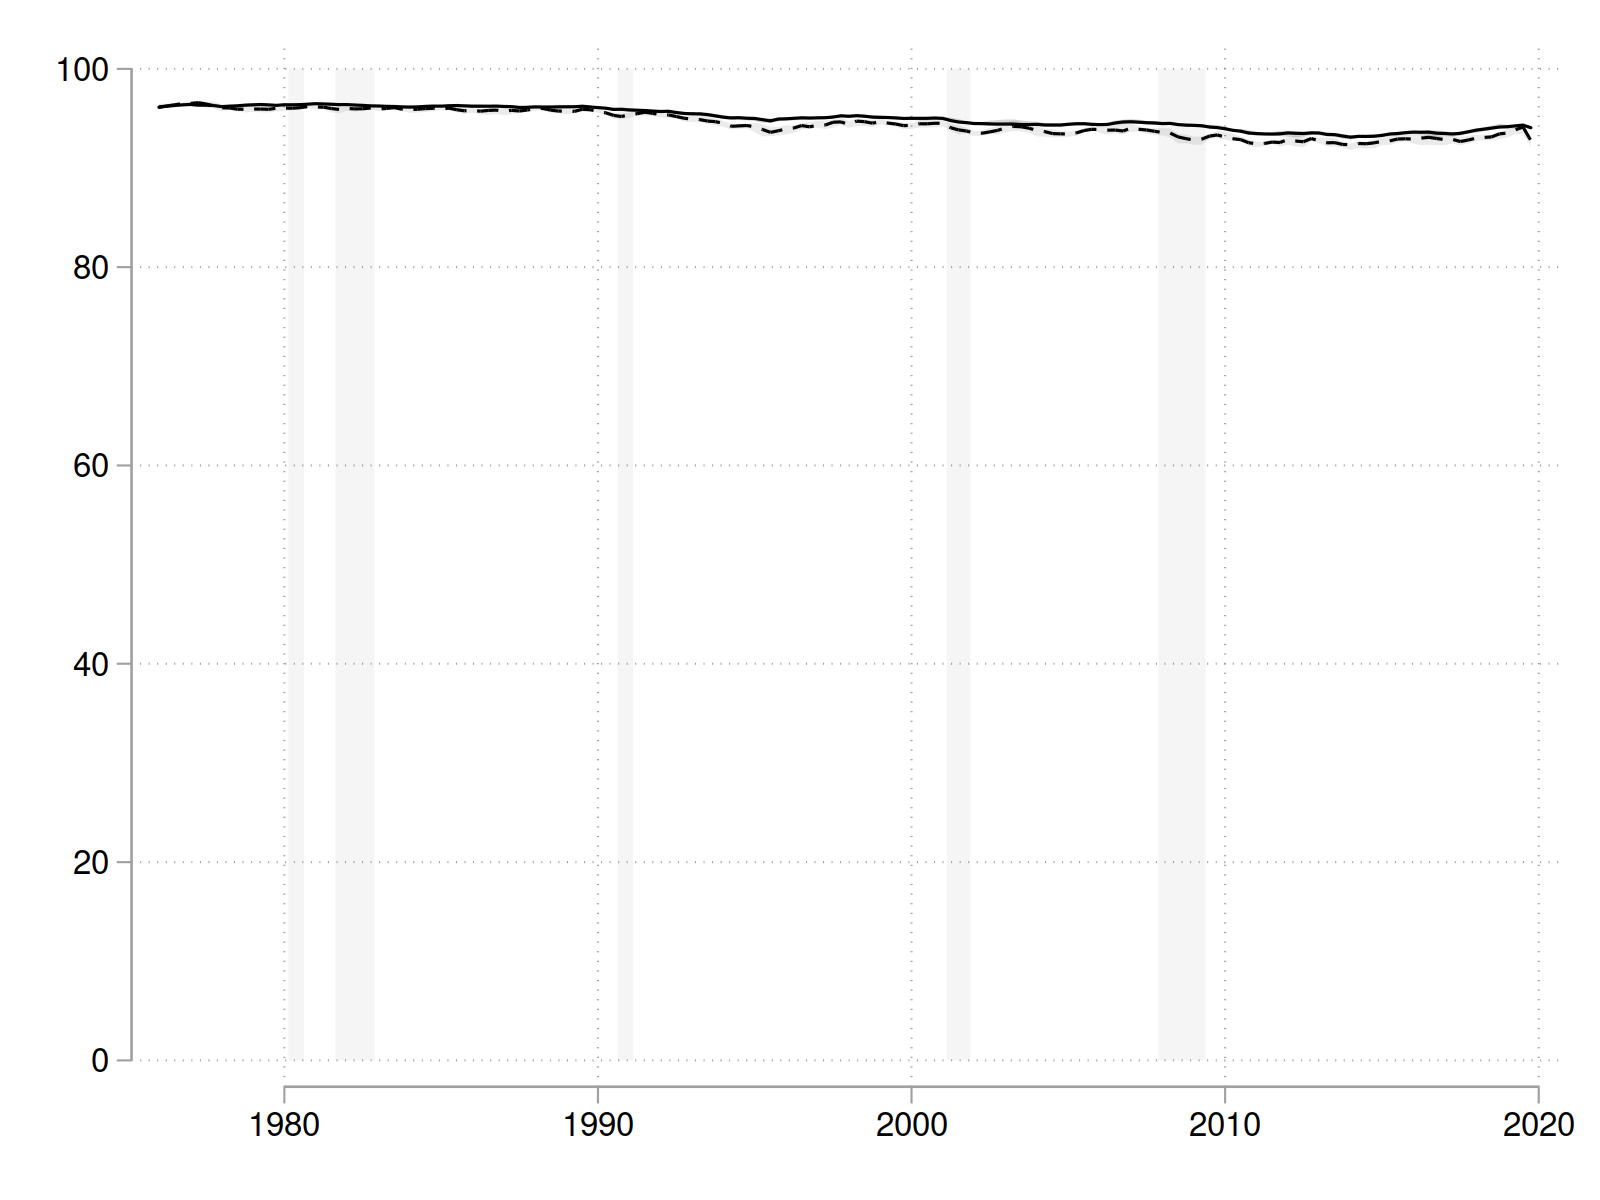
\includegraphics[scale= 0.125]{Y04_QSA_Prate_DeNUN1_sex1_flowtype0.png}
    \caption{Husbands' Participation Rate, $R^2 = 60\%$ }
  \end{subfigure}
  \begin{subfigure}[b]{0.475\textwidth}
    \centering
    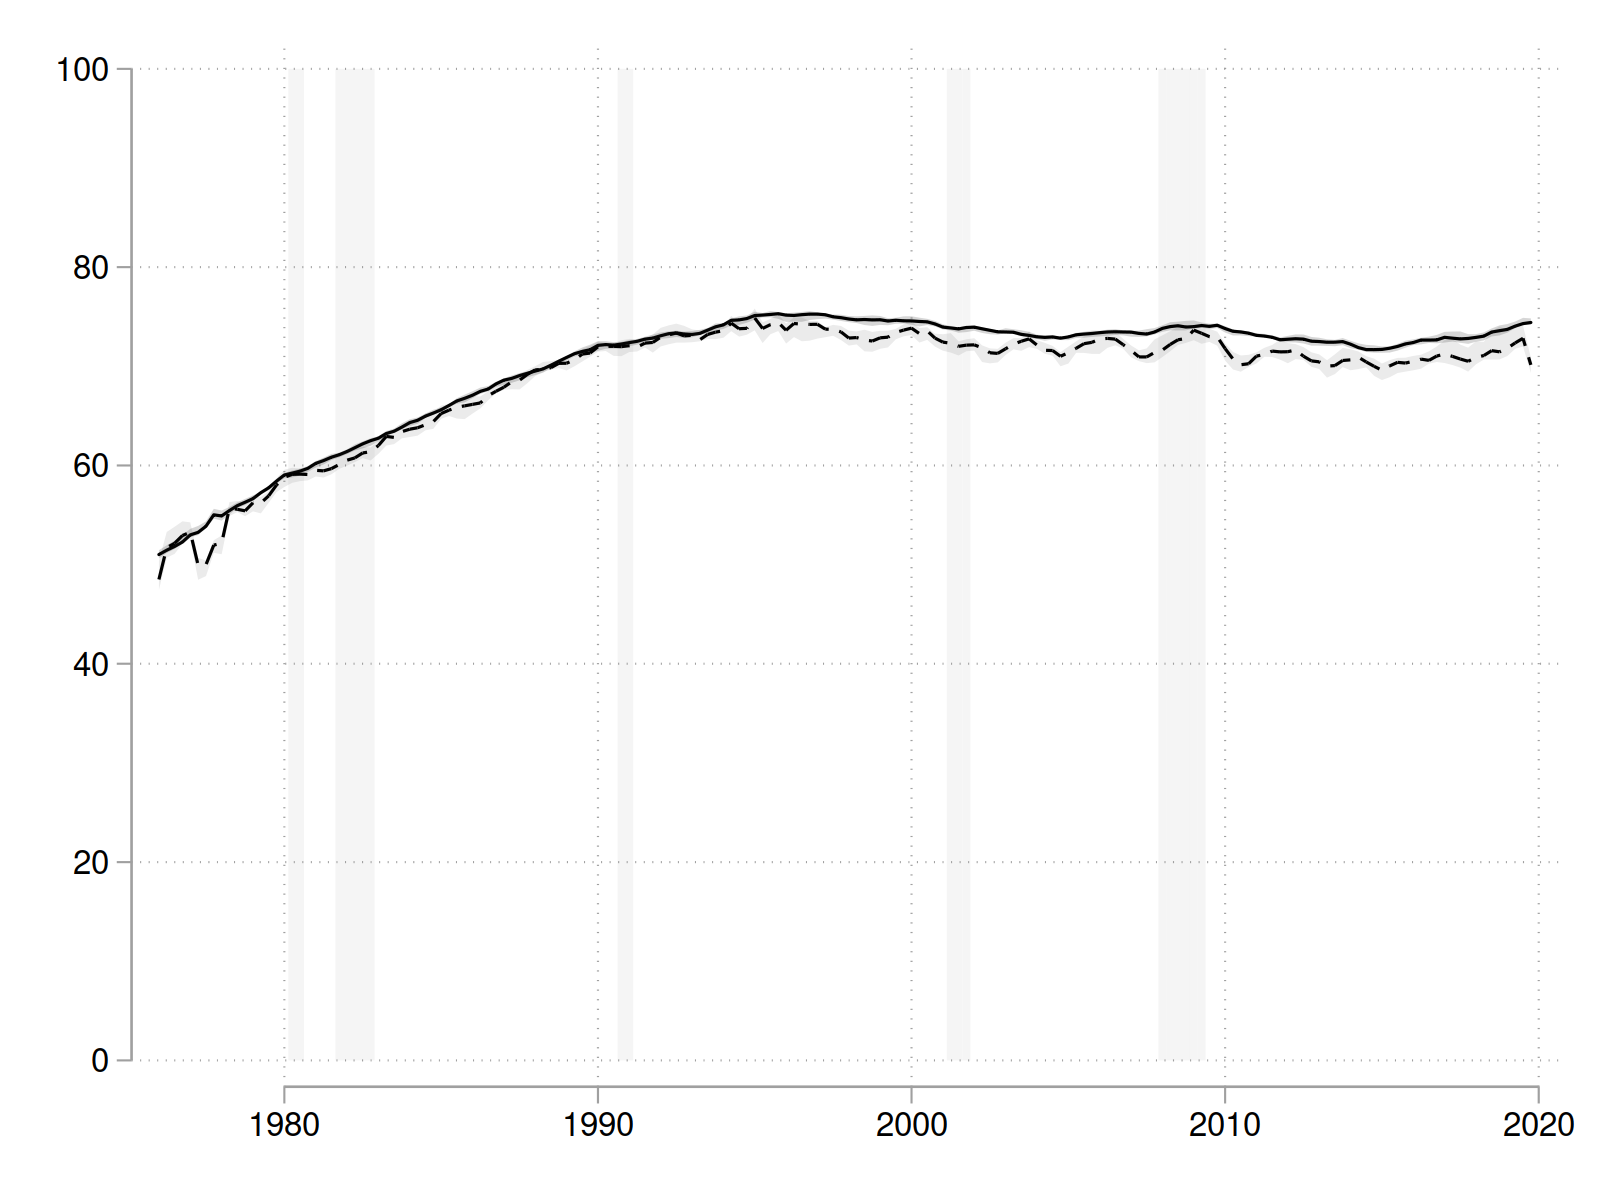
\includegraphics[scale= 0.125]{Y04_QSA_Prate_DeNUN1_sex2_flowtype0.png}
    \caption{Wives' Participation Rate, $R^2 = 94\%$ }
  \end{subfigure}
  \begin{subfigure}[b]{0.475\textwidth}
    \centering
    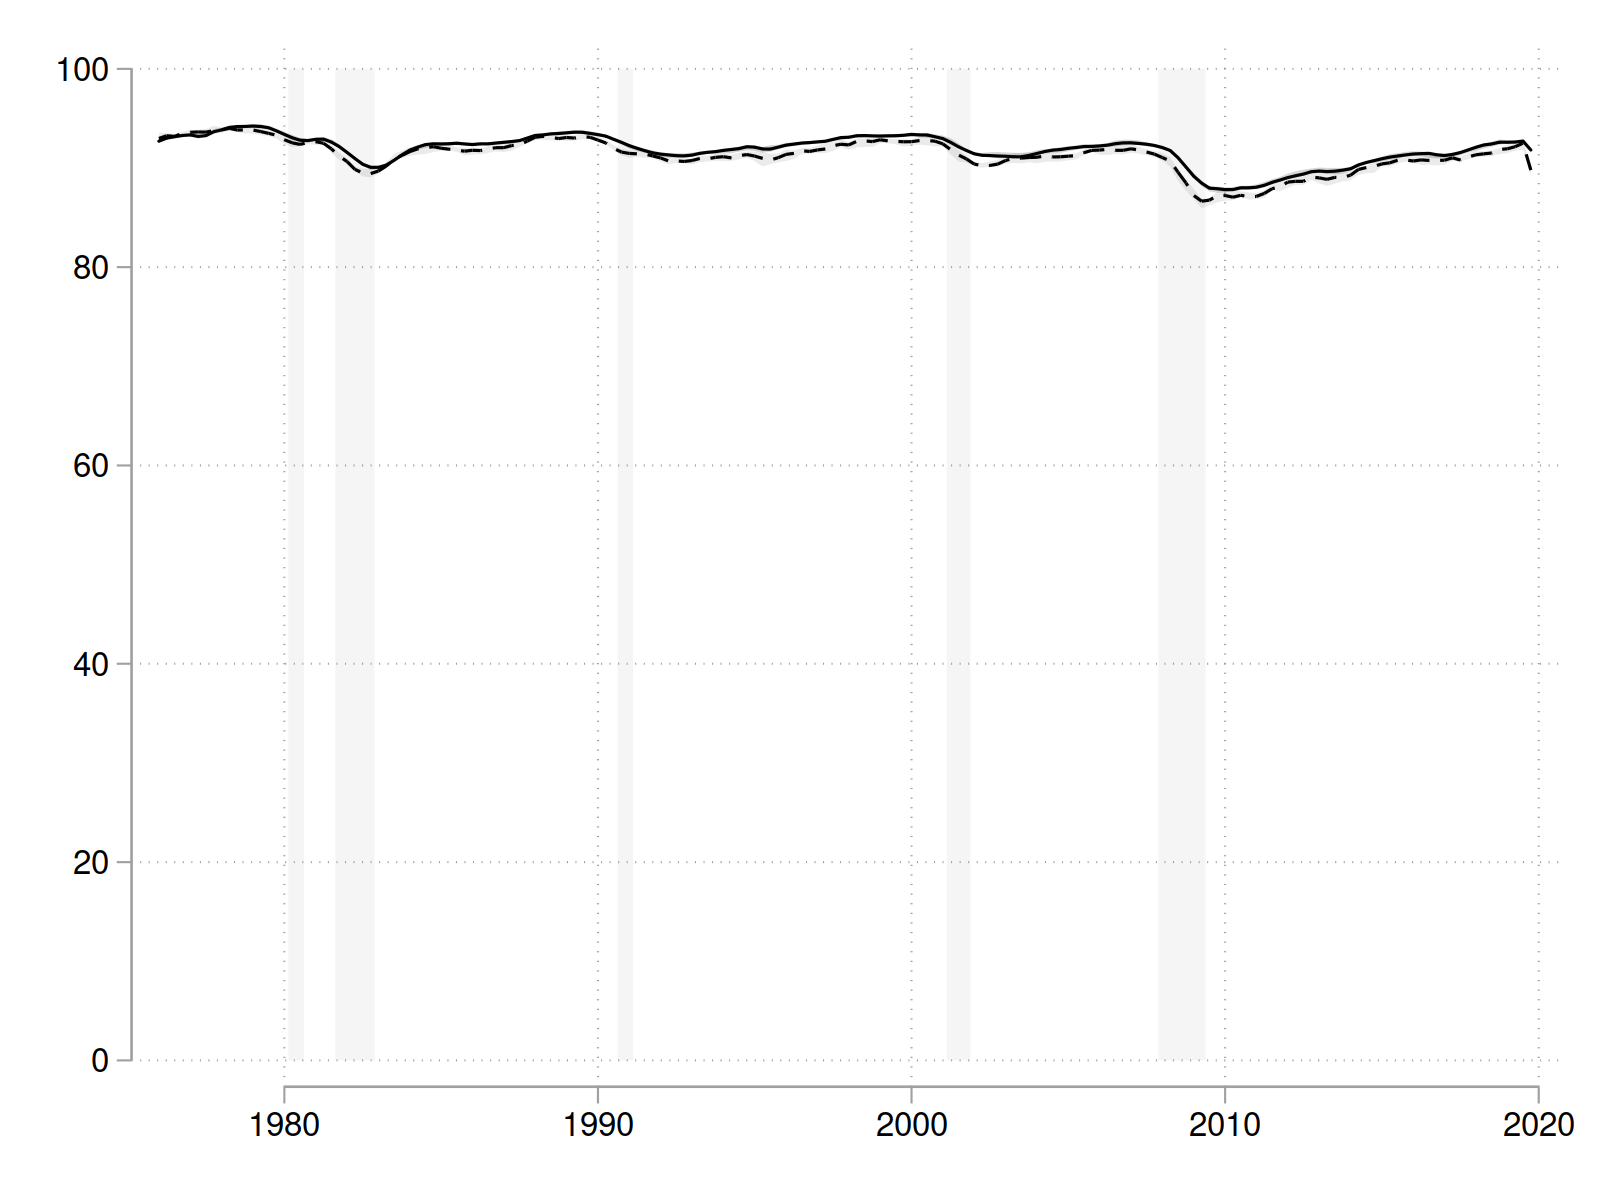
\includegraphics[scale= 0.125]{Y04_QSA_Erate_DeNUN1_sex1_flowtype0.png}
    \caption{Husbands' Employment Rate, $R^2 = 75\%$ }
  \end{subfigure}
  \begin{subfigure}[b]{0.475\textwidth}
    \centering
    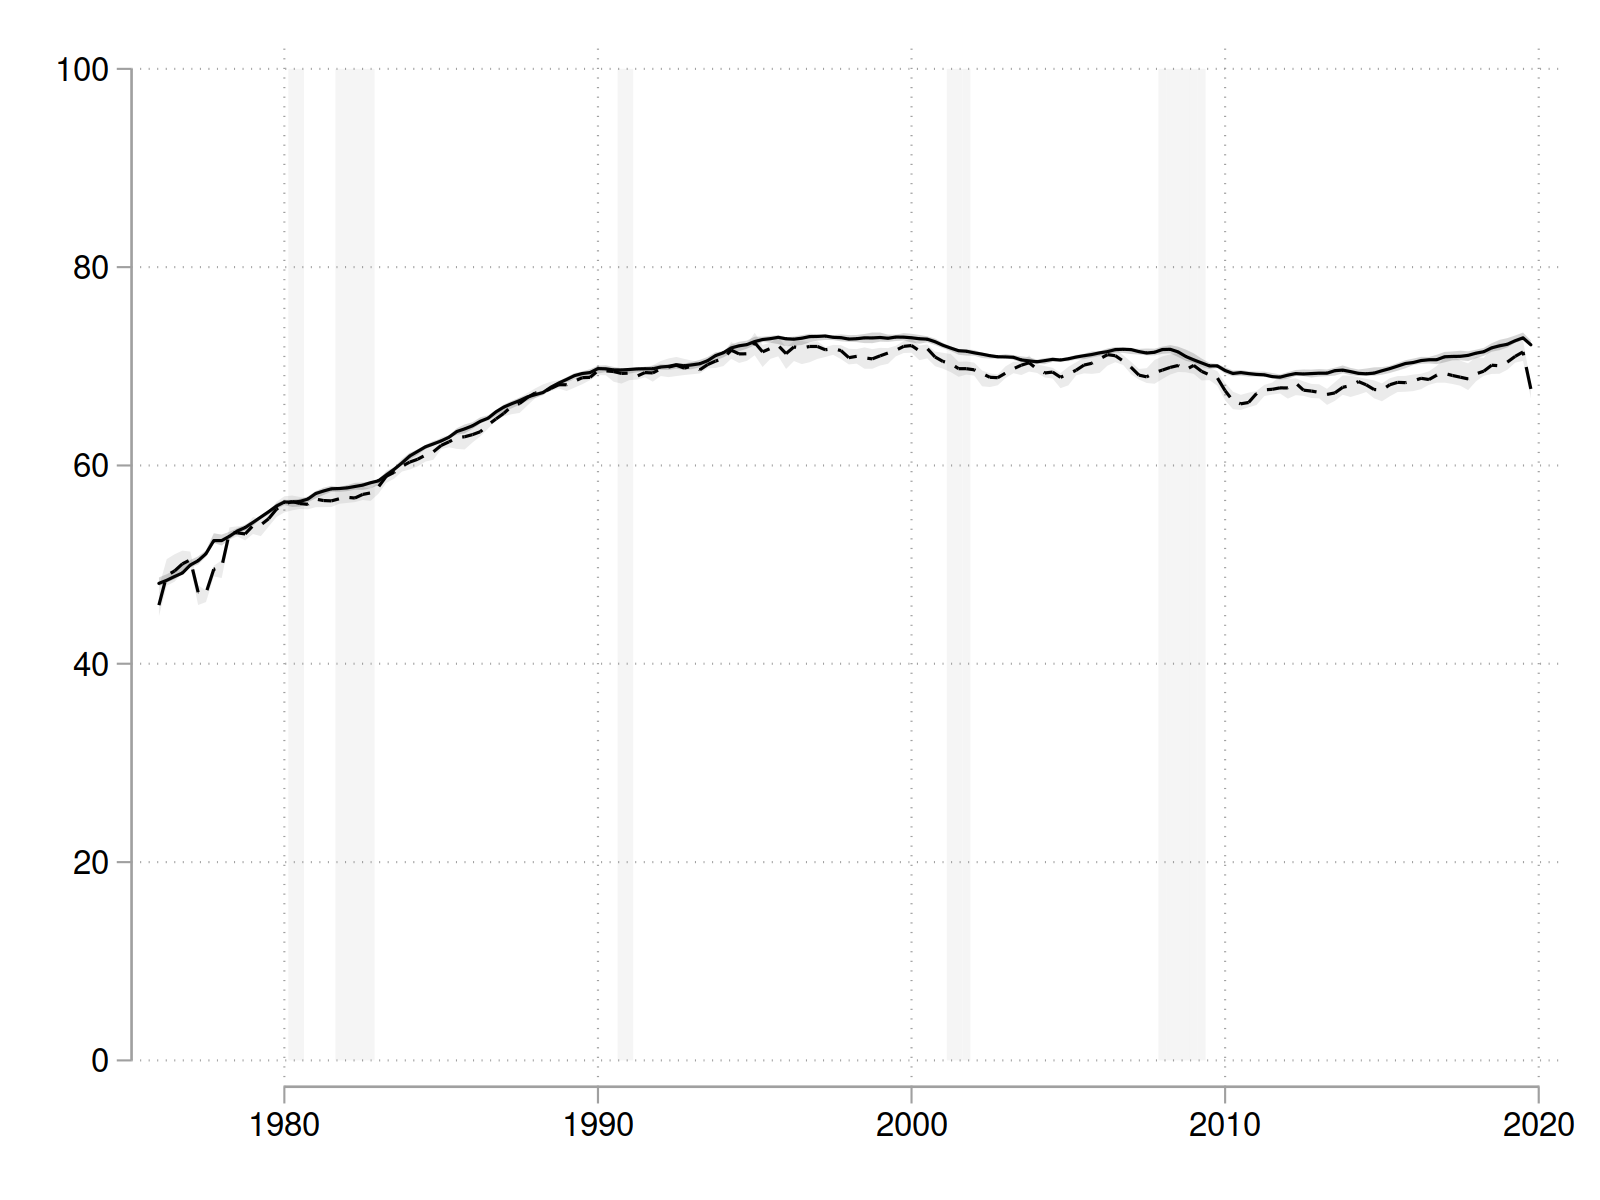
\includegraphics[scale= 0.125]{Y04_QSA_Erate_DeNUN1_sex2_flowtype0.png}
    \caption{Wives' Employment Rate, $R^2 = 94\%$ }
  \end{subfigure}
  \begin{subfigure}[b]{0.475\textwidth}
    \centering
    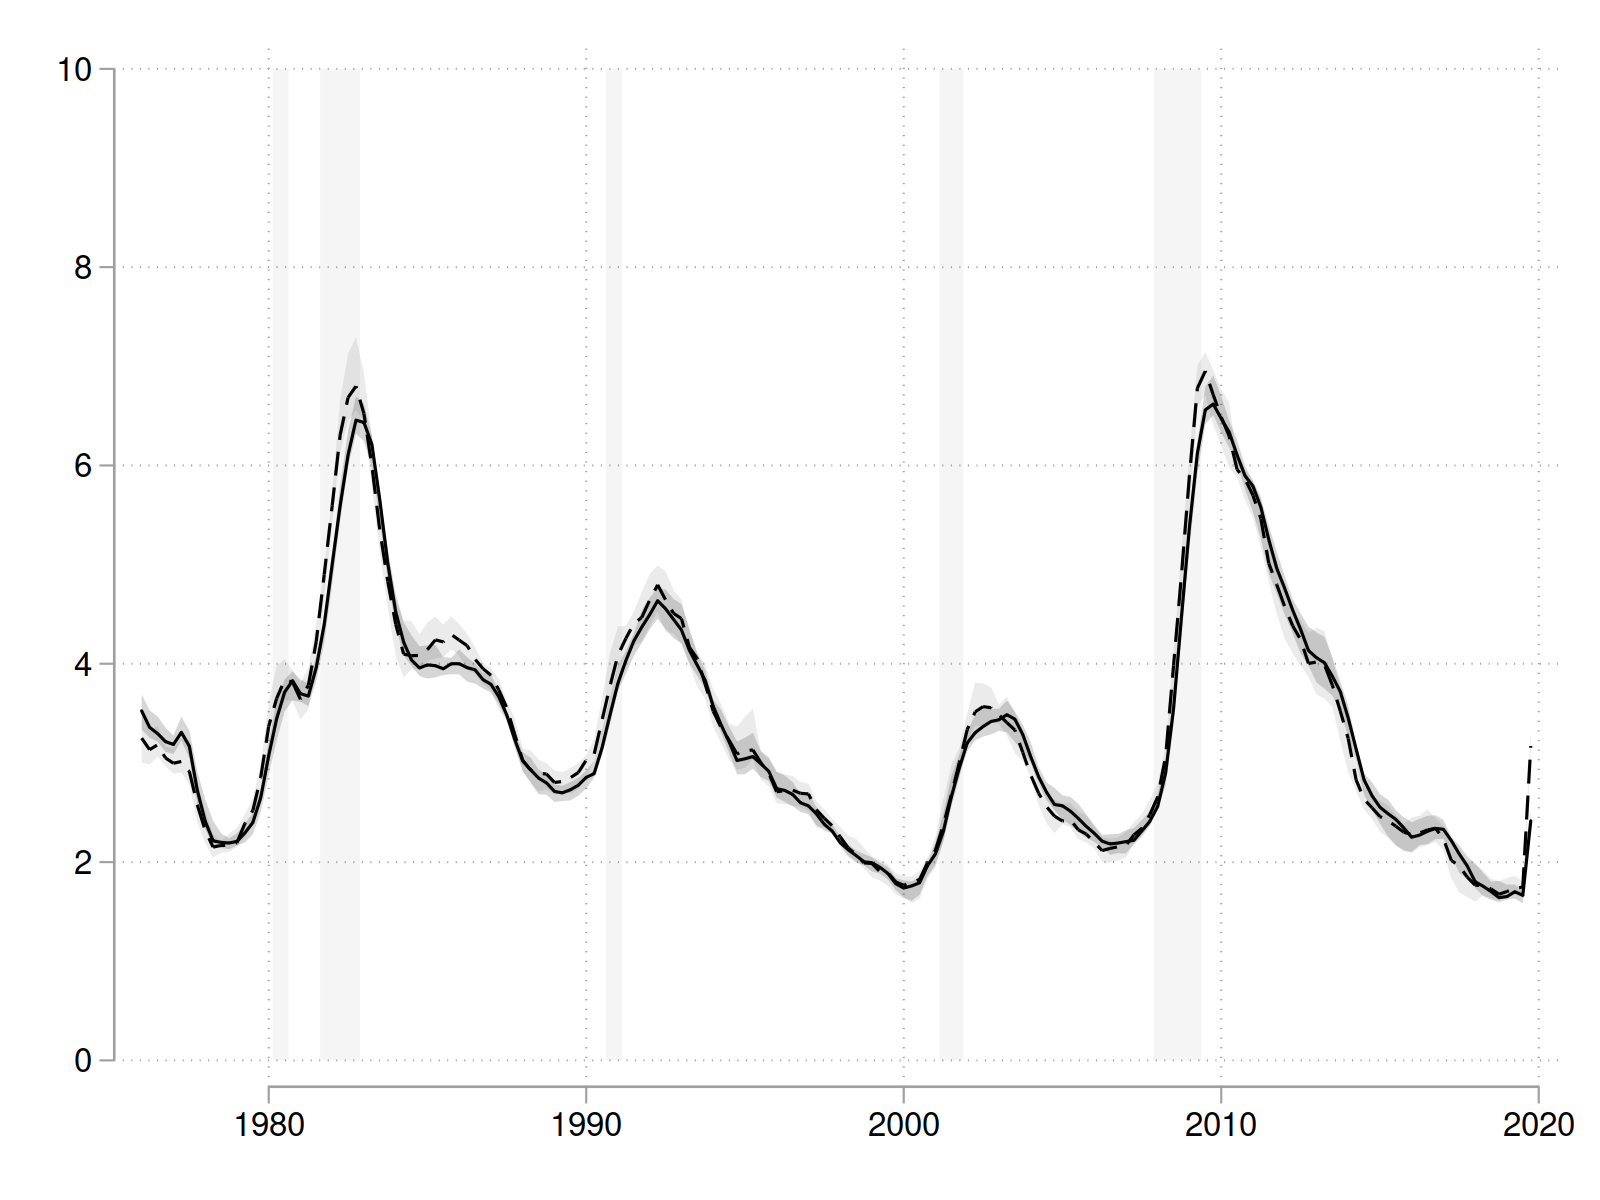
\includegraphics[scale= 0.125]{Y04_QSA_Urate_DeNUN1_sex1_flowtype0.png}
    \caption{Husbands' Unemployment Rate, $R^2 = 97\%$ }
  \end{subfigure}
  \begin{subfigure}[b]{0.475\textwidth}
    \centering
    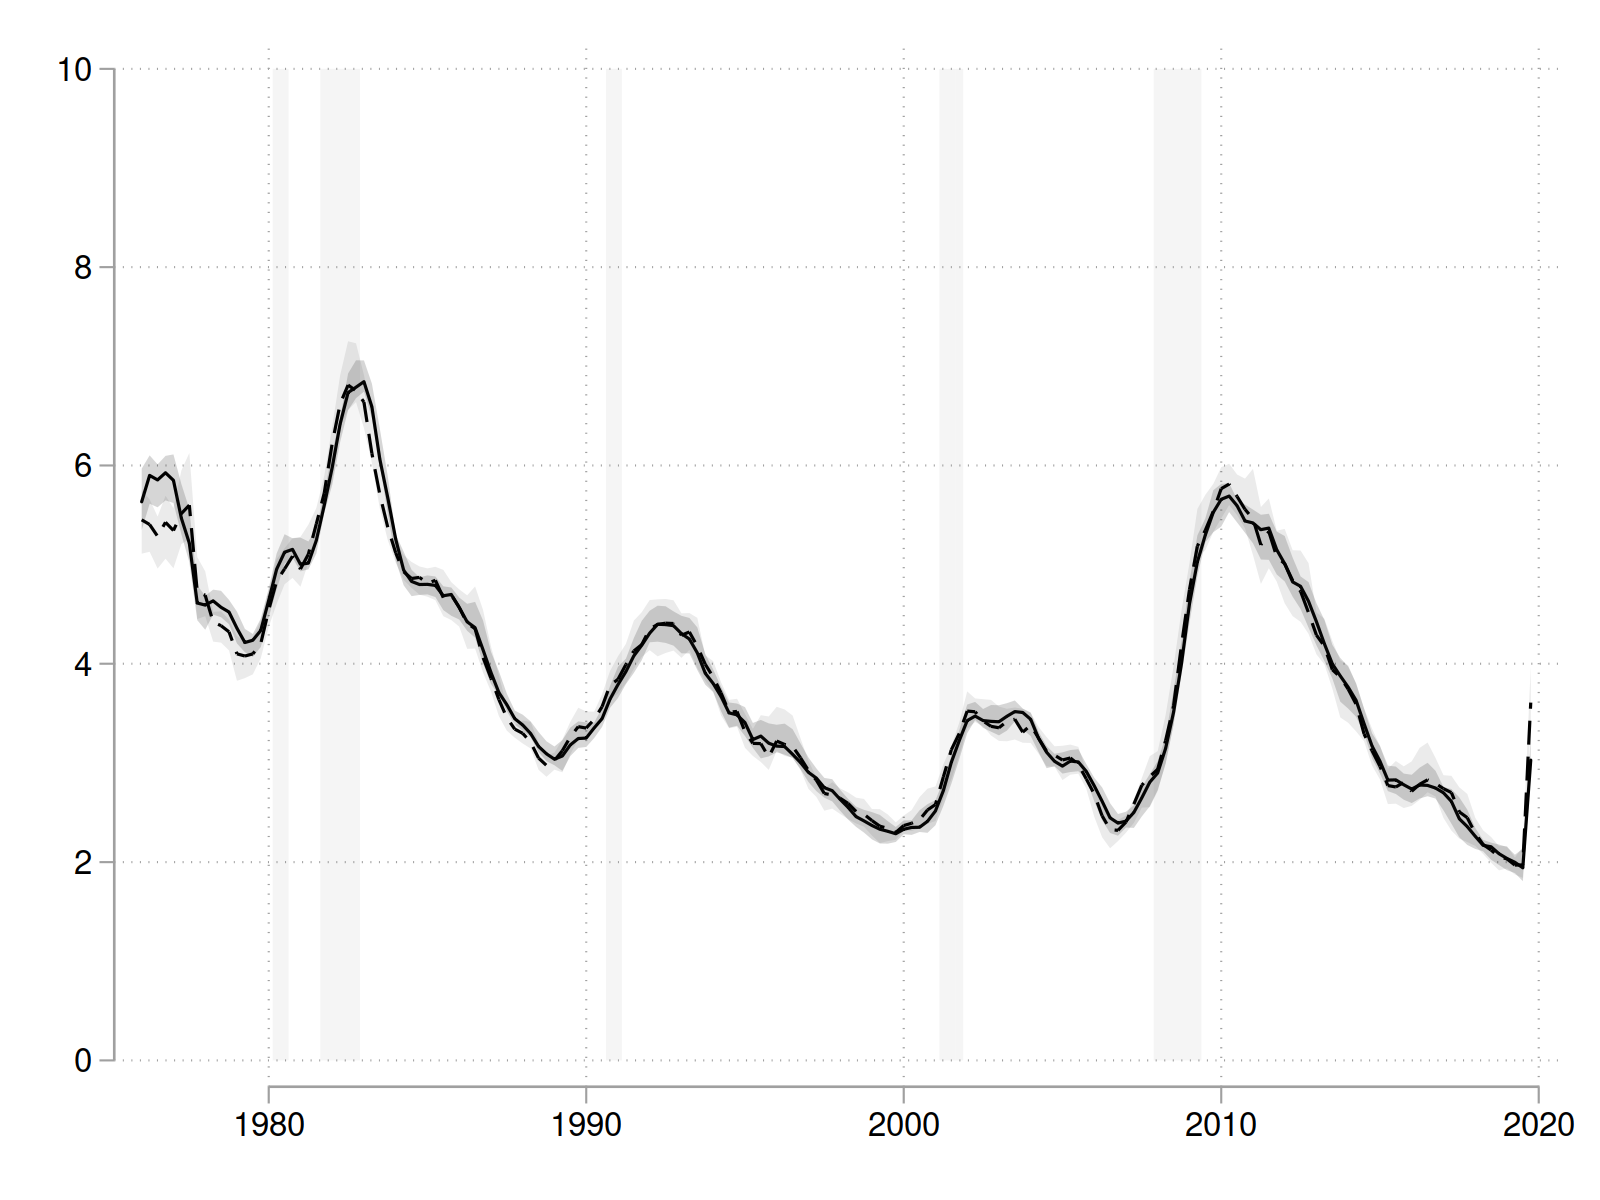
\includegraphics[scale= 0.125]{Y04_QSA_Urate_DeNUN1_sex2_flowtype0.png}
    \caption{Wives' Unemployment Rate, $R^2 = 98\%$ }
  \end{subfigure}
	\floatfoot{\textbf{Notes}:
    CPS 1976:Q1 to 2019:Q4.
    All values are in percent.
    The solid line is the data.
    The dashed line is the steady-state approximation.
    We seasonally adjust monthly estimates using a 12-month moving average and report quarterly averages.
    The data is corrected for classification errors as described in Appendix~Section~A.1.
    Probabilities are corrected for time-aggregation bias as described in Appendix~Section~A.2.
    We report 95\% confidence intervals from 1,000 bootstraps.
    The vertical gray areas are NBER recession periods.
  }
\end{figure}
%----- END FIGURE -----

%----- BEGIN TABLE -----
\begin{table}[H]
	\centering
	\caption{Joint Conditional Transition Probabilities}
  \resizebox{\textwidth}{!}{
\begin{tabular}{>{\centering}m{0.1\textwidth}c|ccc|ccc|ccc}
\hline
\hline
Wife & & \multicolumn{3}{c|}{Husband Employed}
  & \multicolumn{3}{c|}{Husband Unemployed}
  & \multicolumn{3}{c}{Husband Non-participant} \\
Transitions & & E & U & N & E & U & N & E & U & N \\ \hline
\multirow{6}{0.1\textwidth}{\centering Husband Employed}
& \multirow{2}{*}{E}
& 96.24 & 0.78 & 2.97 & 91.69 & 4.28 & 4.03 & 83.26 & 1.43 & 15.31 \\ [-0.1cm] &
& {\scriptsize (96.22, 96.27)} & {\scriptsize (0.77, 0.79)} & {\scriptsize (2.95, 2.99)}
& {\scriptsize (91.34, 92.06)} & {\scriptsize (3.99, 4.54)} & {\scriptsize (3.77, 4.28)}
& {\scriptsize (82.66, 83.82)} & {\scriptsize (1.23, 1.64)} & {\scriptsize (14.76, 15.88)}
\\ [0.1cm]
& \multirow{2}{*}{U}
& 26.23 & 54.84 & 18.93 & 25.11 & 59.72 & 15.17 & 29.12 & 43.89 & 26.99 \\ [-0.1cm] &
& {\scriptsize (25.91, 26.53)} & {\scriptsize (54.49, 55.22)} & {\scriptsize (18.67, 19.20)}
& {\scriptsize (23.33, 26.96)} & {\scriptsize (57.82, 61.79)} & {\scriptsize (13.54, 16.52)}
& {\scriptsize (26.36, 31.84)} & {\scriptsize (40.60, 46.88)} & {\scriptsize (24.27, 29.79)}
\\ [0.1cm]
& \multirow{2}{*}{N}
& 6.11 & 1.63 & 92.26 & 7.56 & 6.01 & 86.42 & 15.19 & 1.57 & 83.24 \\ [-0.1cm] &
& {\scriptsize (6.06, 6.16)} & {\scriptsize (1.60, 1.65)} & {\scriptsize (92.21, 92.32)}
& {\scriptsize (6.98, 8.06)} & {\scriptsize (5.55, 6.50)} & {\scriptsize (85.78, 87.09)}
& {\scriptsize (14.40, 15.98)} & {\scriptsize (1.32, 1.84)} & {\scriptsize (82.38, 84.02)}
\\ [0.1cm]
\hline
\multirow{6}{0.1\textwidth}{\centering Husband Unemployed}
& \multirow{2}{*}{E}
& 94.39 & 1.94 & 3.67 & 96.27 & 1.84 & 1.89 & 94.61 & 1.32 & 4.07 \\ [-0.1cm] &
& {\scriptsize (94.09, 94.69)} & {\scriptsize (1.77, 2.11)} & {\scriptsize (3.43, 3.91)}
& {\scriptsize (96.09, 96.45)} & {\scriptsize (1.72, 1.96)} & {\scriptsize (1.77, 2.02)}
& {\scriptsize (93.99, 95.32)} & {\scriptsize (1.00, 1.64)} & {\scriptsize (3.46, 4.68)}
\\ [0.1cm]
& \multirow{2}{*}{U}
& 35.68 & 45.82 & 18.50 & 16.65 & 70.51 & 12.84 & 20.77 & 37.95 & 41.28 \\ [-0.1cm] &
& {\scriptsize (33.95, 37.52)} & {\scriptsize (44.14, 47.98)} & {\scriptsize (16.77, 19.78)}
& {\scriptsize (15.55, 17.66)} & {\scriptsize (69.36, 71.92)} & {\scriptsize (12.03, 13.72)}
& {\scriptsize (18.36, 23.94)} & {\scriptsize (34.34, 40.86)} & {\scriptsize (37.93, 44.70)}
\\ [0.1cm]
& \multirow{2}{*}{N}
& 8.53 & 3.60 & 87.87 & 4.56 & 5.67 & 89.77 & 5.75 & 2.76 & 91.49 \\ [-0.1cm] &
& {\scriptsize (7.94, 9.11)} & {\scriptsize (3.22, 3.97)} & {\scriptsize (87.25, 88.57)}
& {\scriptsize (4.24, 4.89)} & {\scriptsize (5.33, 6.01)} & {\scriptsize (89.31, 90.23)}
& {\scriptsize (4.88, 6.79)} & {\scriptsize (2.09, 3.46)} & {\scriptsize (90.29, 92.60)}
\\ [0.1cm]
\hline
\multirow{6}{0.1\textwidth}{\centering Husband Non-participant}
& \multirow{2}{*}{E}
& 89.28 & 1.31 & 9.41 & 95.72 & 2.15 & 2.13 & 96.18 & 1.13 & 2.69 \\ [-0.1cm] &
& {\scriptsize (88.80, 89.81)} & {\scriptsize (1.12, 1.52)} & {\scriptsize (8.90, 9.89)}
& {\scriptsize (95.14, 96.25)} & {\scriptsize (1.77, 2.54)} & {\scriptsize (1.73, 2.57)}
& {\scriptsize (96.06, 96.30)} & {\scriptsize (1.06, 1.20)} & {\scriptsize (2.58, 2.79)}
\\ [0.1cm]
& \multirow{2}{*}{U}
& 32.87 & 48.07 & 19.06 & 20.18 & 63.21 & 16.60 & 21.07 & 58.42 & 20.51 \\ [-0.1cm] &
& {\scriptsize (29.96, 36.55)} & {\scriptsize (44.56, 51.54)} & {\scriptsize (16.03, 21.44)}
& {\scriptsize (16.27, 23.17)} & {\scriptsize (59.03, 67.94)} & {\scriptsize (13.67, 19.84)}
& {\scriptsize (19.91, 22.24)} & {\scriptsize (56.78, 59.91)} & {\scriptsize (19.44, 21.70)}
\\ [0.1cm]
& \multirow{2}{*}{N}
& 23.97 & 2.82 & 73.21 & 6.75 & 10.65 & 82.60 & 3.24 & 1.40 & 95.36 \\ [-0.1cm] &
& {\scriptsize (23.12, 24.86)} & {\scriptsize (2.47, 3.18)} & {\scriptsize (72.24, 74.13)}
& {\scriptsize (5.82, 7.72)} & {\scriptsize (9.34, 11.70)} & {\scriptsize (81.34, 84.15)}
& {\scriptsize (3.11, 3.38)} & {\scriptsize (1.31, 1.49)} & {\scriptsize (95.19, 95.52)}
\\ [0.1cm]
\hline
\hline
\end{tabular}
}

  \\ \bigskip
  \resizebox{\textwidth}{!}{
\begin{tabular}{>{\centering}m{0.1\textwidth}c|ccc|ccc|ccc}
\hline
\hline
Husband & & \multicolumn{3}{c|}{Wife Employed}
  & \multicolumn{3}{c|}{Wife Unemployed}
  & \multicolumn{3}{c}{Wife Non-participant} \\
Transitions & & E & U & N & E & U & N & E & U & N \\ \hline
\multirow{6}{0.1\textwidth}{\centering Wife Employed}
& \multirow{2}{*}{E}
& 98.62 & 0.88 & 0.50 & 94.15 & 4.78 & 1.07 & 95.32 & 1.25 & 3.43 \\ [-0.1cm] &
& {\scriptsize (98.60, 98.63)} & {\scriptsize (0.87, 0.89)} & {\scriptsize (0.50, 0.51)}
& {\scriptsize (93.83, 94.47)} & {\scriptsize (4.48, 5.04)} & {\scriptsize (0.93, 1.23)}
& {\scriptsize (95.16, 95.46)} & {\scriptsize (1.18, 1.33)} & {\scriptsize (3.30, 3.57)}
\\ [0.1cm]
& \multirow{2}{*}{U}
& 29.22 & 63.67 & 7.11 & 31.96 & 63.99 & 4.05 & 42.43 & 45.88 & 11.69 \\ [-0.1cm] &
& {\scriptsize (28.86, 29.58)} & {\scriptsize (63.28, 64.05)} & {\scriptsize (6.92, 7.31)}
& {\scriptsize (29.53, 34.26)} & {\scriptsize (61.60, 66.56)} & {\scriptsize (3.17, 5.18)}
& {\scriptsize (40.29, 44.48)} & {\scriptsize (43.72, 48.16)} & {\scriptsize (10.24, 13.12)}
\\ [0.1cm]
& \multirow{2}{*}{N}
& 10.01 & 4.52 & 85.47 & 11.24 & 8.69 & 80.07 & 29.33 & 3.07 & 67.59 \\ [-0.1cm] &
& {\scriptsize (9.82, 10.21)} & {\scriptsize (4.38, 4.66)} & {\scriptsize (85.23, 85.70)}
& {\scriptsize (9.95, 13.15)} & {\scriptsize (7.17, 9.87)} & {\scriptsize (77.91, 81.82)}
& {\scriptsize (27.83, 30.80)} & {\scriptsize (2.50, 3.64)} & {\scriptsize (66.20, 69.13)}
\\ [0.1cm]
\hline
\multirow{6}{0.1\textwidth}{\centering Wife Unemployed}
& \multirow{2}{*}{E}
& 96.83 & 2.20 & 0.98 & 96.89 & 2.46 & 0.64 & 97.03 & 1.78 & 1.20 \\ [-0.1cm] &
& {\scriptsize (96.59, 97.06)} & {\scriptsize (2.00, 2.39)} & {\scriptsize (0.83, 1.11)}
& {\scriptsize (96.74, 97.04)} & {\scriptsize (2.34, 2.59)} & {\scriptsize (0.57, 0.71)}
& {\scriptsize (96.77, 97.26)} & {\scriptsize (1.59, 1.97)} & {\scriptsize (1.03, 1.37)}
\\ [0.1cm]
& \multirow{2}{*}{U}
& 44.48 & 49.93 & 5.59 & 20.99 & 75.21 & 3.80 & 30.55 & 53.04 & 16.42 \\ [-0.1cm] &
& {\scriptsize (41.99, 46.23)} & {\scriptsize (48.00, 52.28)} & {\scriptsize (4.80, 6.78)}
& {\scriptsize (19.81, 22.15)} & {\scriptsize (74.01, 76.61)} & {\scriptsize (3.23, 4.28)}
& {\scriptsize (28.24, 32.47)} & {\scriptsize (50.82, 55.38)} & {\scriptsize (14.81, 18.50)}
\\ [0.1cm]
& \multirow{2}{*}{N}
& 13.06 & 6.28 & 80.66 & 7.18 & 6.54 & 86.28 & 8.24 & 4.76 & 87.00 \\ [-0.1cm] &
& {\scriptsize (11.69, 15.06)} & {\scriptsize (4.71, 7.18)} & {\scriptsize (78.65, 82.77)}
& {\scriptsize (6.34, 8.18)} & {\scriptsize (5.72, 7.27)} & {\scriptsize (85.00, 87.47)}
& {\scriptsize (6.81, 9.59)} & {\scriptsize (3.94, 6.14)} & {\scriptsize (85.14, 88.46)}
\\ [0.1cm]
\hline
\multirow{6}{0.1\textwidth}{\centering Wife Non-participant}
& \multirow{2}{*}{E}
& 96.65 & 1.26 & 2.09 & 95.53 & 3.77 & 0.70 & 98.37 & 0.97 & 0.65 \\ [-0.1cm] &
& {\scriptsize (96.50, 96.80)} & {\scriptsize (1.18, 1.35)} & {\scriptsize (1.96, 2.20)}
& {\scriptsize (95.20, 95.82)} & {\scriptsize (3.50, 4.05)} & {\scriptsize (0.57, 0.83)}
& {\scriptsize (98.35, 98.40)} & {\scriptsize (0.95, 0.99)} & {\scriptsize (0.64, 0.67)}
\\ [0.1cm]
& \multirow{2}{*}{U}
& 44.29 & 48.15 & 7.56 & 24.11 & 71.19 & 4.70 & 31.10 & 60.51 & 8.39 \\ [-0.1cm] &
& {\scriptsize (42.20, 46.46)} & {\scriptsize (45.83, 50.05)} & {\scriptsize (6.51, 8.96)}
& {\scriptsize (21.77, 25.89)} & {\scriptsize (69.29, 73.75)} & {\scriptsize (3.65, 5.89)}
& {\scriptsize (30.51, 31.72)} & {\scriptsize (59.87, 61.19)} & {\scriptsize (8.00, 8.76)}
\\ [0.1cm]
& \multirow{2}{*}{N}
& 43.58 & 4.46 & 51.96 & 14.94 & 18.79 & 66.26 & 7.89 & 3.14 & 88.97 \\ [-0.1cm] &
& {\scriptsize (42.04, 45.11)} & {\scriptsize (3.80, 5.12)} & {\scriptsize (50.47, 53.53)}
& {\scriptsize (13.43, 16.79)} & {\scriptsize (17.04, 20.89)} & {\scriptsize (63.67, 68.26)}
& {\scriptsize (7.68, 8.10)} & {\scriptsize (3.01, 3.27)} & {\scriptsize (88.72, 89.22)}
\\ [0.1cm]
\hline
\hline
\end{tabular}
}

	\floatfoot{\textbf{Notes}:
    CPS 1976 to 2019.
    All values are in percent.
    Each sub-panel represents the transition probabilities of husbands (upper panel) or wives (lower panel) conditional on the transitions of wives or husbands, respectively.
    Rows correspond to states in period $t-1$, columns in period $t$.
    We seasonally adjust monthly estimates using a 12-month moving average and report quarterly averages.
    The data is corrected for classification errors as described in Appendix~Section~A.1.
    Probabilities are corrected for time-aggregation bias as described in Appendix~Section~A.2.
    We report 95\% confidence intervals from 1,000 bootstraps.
	}
\end{table}
%----- END TABLE -----

%----- BEGIN TABLE -----
\begin{table}[H]
  \centering
  \caption{Decomposed Flows}
  \begin{tabular}{c|c|c|c}
  \hline \hline
  $t-1$, $t$ & $E$      & $U$      & $N$      \\ \hline
  $E$        & $f_{EE}$ & $f_{EU}$ & $f_{EN}$ \\ \hline
  $U$        & $f_{UE}$ & $f_{UU}$ & $f_{UN}$ \\ \hline
  $N$        & $f_{NE|EU} + f_{NE|\neg EU}$
             & $f_{NU|EU} + f_{NU|\neg EU}$
             & $f_{NN|EU} + f_{NN|\neg EU}$
             \\ \hline \hline
\end{tabular}

\end{table}
%----- END TABLE ----

%----- BEGIN TABLE -----
\begin{table}[H]
  \centering
  \caption{Counterfactual Transition Rates}
  \renewcommand{\arraystretch}{2}
  \begin{tabular}{c|c|c|c}
  \hline \hline
  $t-1$, $t$ & $E$      & $U$      & $N$      \\ \hline
  $E$        & $\frac{f_{EE}}{f_{EE}+f_{EU}+f_{EN}}$
             & $\frac{f_{EU}}{f_{EE}+f_{EU}+f_{EN}}$
             & $\frac{f_{EN}}{f_{EE}+f_{EU}+f_{EN}}$
             \\ \hline
  $U$        & $\frac{f_{UE}}{f_{UE}+f_{UU}+f_{UN}}$
             & $\frac{f_{UU}}{f_{UE}+f_{UU}+f_{UN}}$
             & $\frac{f_{UN}}{f_{UE}+f_{UU}+f_{UN}}$
             \\ \hline
  $N$        & $\frac{f_{NE|\neg EU}}{f_{NE}+f_{NU}+f_{NN}}$
             & $\frac{f_{NU|\neg EU}}{f_{NE}+f_{NU}+f_{NN}}$
             & $\frac{f_{NN} + f_{NE|EU} + f_{NU|EU}}{f_{NE}+f_{NU}+f_{NN}}$
             \\ \hline \hline
\end{tabular}

\end{table}
%----- END TABLE ----

%----- BEGIN FIGURE -----
\begin{figure}[H]
  \centering
  \caption{The Aggregate AWE, Married Women}
  \foreach \r\rname in {P/Participation, E/Employment, U/Unemployment}{
  \foreach \rw\rwname in {32/Contemporaneous Effect, 34/Effect with Leads and Lags}{
    \begin{subfigure}[b]{0.45\textwidth}
      \centering
      \includegraphics[scale= 0.125]{Y05_CFs_diffTQSA_sex2_DeNUN1_transtype\rw _diff\r rate.png}%
      \caption{\rname , \rwname}
    \end{subfigure}%
  }
  }
  \floatfoot{\textbf{Notes}:
    CPS 1976:Q1 to 2021:Q4.
    All values are the difference, in percentage points, between the steady-state approximation of the data and the counterfactual steady-state.
    In the counterfactual, added workers do not enter the labor market and remain classified as non-participants.
    We include all spouses who move from employment to unemployment.
    We seasonally adjust monthly estimates using a ratio to moving average.
    The data is corrected for classification errors as described in Appendix~Section~A.1.
    Probabilities are corrected for time-aggregation bias as described in Appendix~Section~A.2.
    We report 95\% confidence intervals from 1,000 bootstraps.
    The vertical gray areas are NBER recession periods.
  }
\end{figure}
%----- END FIGURE -----

%----- BEGIN TABLE -----
\begin{table}[H]
  \centering
  \caption{The Aggregate AWE, Married Women, Participation}
  \def\arraystretch{1.25}
  \resizebox{\textwidth}{!}{
\begin{tabular}{l|c|c|c|c|c|c|c|c|c}
\hline
\hline
& 1976 & & & 1976 & 1980 & 1990 & 2000 & 2010 & 2020 \\
& to & Expansions & Recessions & to & to & to & to & to & to \\
& 2019 & & & 1979 & 1989 & 1999 & 2009 & 2019 & 2021 \\
\hline
SS
& 68.971 & 69.132 & 67.610 & 54.425 & 64.695 & 73.203 & 72.235 & 70.934 & 71.530 \\
& {\scriptsize (68.805, 69.127)}
& {\scriptsize (68.959, 69.300)}
& {\scriptsize (67.181, 68.036)}
& {\scriptsize (53.887, 55.014)}
& {\scriptsize (64.384, 65.011)}
& {\scriptsize (72.914, 73.512)}
& {\scriptsize (71.900, 72.557)}
& {\scriptsize (70.576, 71.333)}
& {\scriptsize (70.545, 72.481)}
\\ [0.1cm]
\hline
\noalign{\smallskip}
\multicolumn{10}{l}{\textbf{Contemporaneous Effect}} \\
\noalign{\smallskip}
\hline
Mean
& 0.306 & 0.294 & 0.411 & 0.278 & 0.367 & 0.308 & 0.278 & 0.279 & 0.406 \\
& {\scriptsize (0.289, 0.323)}
& {\scriptsize (0.276, 0.311)}
& {\scriptsize (0.358, 0.471)}
& {\scriptsize (0.233, 0.328)}
& {\scriptsize (0.336, 0.399)}
& {\scriptsize (0.276, 0.342)}
& {\scriptsize (0.246, 0.316)}
& {\scriptsize (0.239, 0.321)}
& {\scriptsize (0.258, 0.560)}
\\ [0.1cm]
\hline
Max
& 0.915 & 0.876 & 0.783 & 0.496 & 0.715 & 0.705 & 0.755 & 0.850 & 1.617 \\
& {\scriptsize (0.724, 1.306)}
& {\scriptsize (0.696, 1.294)}
& {\scriptsize (0.606, 1.090)}
& {\scriptsize (0.372, 0.716)}
& {\scriptsize (0.588, 0.931)}
& {\scriptsize (0.562, 0.963)}
& {\scriptsize (0.555, 1.087)}
& {\scriptsize (0.614, 1.294)}
& {\scriptsize (0.815, 2.555)}
\\ [0.1cm]
\hline
P25
& 0.187 & 0.178 & 0.256 & 0.197 & 0.261 & 0.186 & 0.165 & 0.137 & 0.107 \\
& {\scriptsize (0.164, 0.210)}
& {\scriptsize (0.155, 0.204)}
& {\scriptsize (0.186, 0.331)}
& {\scriptsize (0.136, 0.259)}
& {\scriptsize (0.223, 0.302)}
& {\scriptsize (0.145, 0.224)}
& {\scriptsize (0.124, 0.210)}
& {\scriptsize (0.092, 0.183)}
& {\scriptsize (0.040, 0.200)}
\\ [0.1cm]
\hline
P75
& 0.403 & 0.388 & 0.543 & 0.353 & 0.458 & 0.416 & 0.358 & 0.381 & 0.419 \\
& {\scriptsize (0.371, 0.434)}
& {\scriptsize (0.358, 0.422)}
& {\scriptsize (0.445, 0.650)}
& {\scriptsize (0.275, 0.443)}
& {\scriptsize (0.402, 0.514)}
& {\scriptsize (0.354, 0.485)}
& {\scriptsize (0.303, 0.426)}
& {\scriptsize (0.317, 0.463)}
& {\scriptsize (0.257, 0.667)}
\\ [0.1cm]
\hline
\noalign{\smallskip}
\multicolumn{10}{l}{\textbf{Effect with Leads and Lags}} \\
\noalign{\smallskip}
\hline
Mean
& 0.721 & 0.697 & 0.928 & 0.576 & 0.871 & 0.684 & 0.667 & 0.708 & 1.026 \\
& {\scriptsize (0.694, 0.748)}
& {\scriptsize (0.668, 0.725)}
& {\scriptsize (0.841, 1.013)}
& {\scriptsize (0.507, 0.650)}
& {\scriptsize (0.822, 0.922)}
& {\scriptsize (0.632, 0.734)}
& {\scriptsize (0.609, 0.721)}
& {\scriptsize (0.646, 0.781)}
& {\scriptsize (0.642, 1.295)}
\\ [0.1cm]
\hline
Max
& 1.808 & 1.735 & 1.619 & 0.990 & 1.606 & 1.345 & 1.416 & 1.703 & 2.957 \\
& {\scriptsize (1.508, 2.359)}
& {\scriptsize (1.415, 2.359)}
& {\scriptsize (1.319, 2.108)}
& {\scriptsize (0.782, 1.352)}
& {\scriptsize (1.324, 2.031)}
& {\scriptsize (1.088, 1.860)}
& {\scriptsize (1.095, 1.939)}
& {\scriptsize (1.324, 2.359)}
& {\scriptsize (1.800, 4.368)}
\\ [0.1cm]
\hline
P25
& 0.513 & 0.504 & 0.638 & 0.437 & 0.672 & 0.508 & 0.474 & 0.449 & 0.428 \\
& {\scriptsize (0.477, 0.549)}
& {\scriptsize (0.467, 0.541)}
& {\scriptsize (0.496, 0.794)}
& {\scriptsize (0.327, 0.531)}
& {\scriptsize (0.599, 0.749)}
& {\scriptsize (0.441, 0.582)}
& {\scriptsize (0.405, 0.551)}
& {\scriptsize (0.362, 0.542)}
& {\scriptsize (0.231, 0.647)}
\\ [0.1cm]
\hline
P75
& 0.891 & 0.859 & 1.182 & 0.703 & 1.033 & 0.831 & 0.827 & 0.910 & 1.337 \\
& {\scriptsize (0.839, 0.941)}
& {\scriptsize (0.811, 0.909)}
& {\scriptsize (1.029, 1.356)}
& {\scriptsize (0.582, 0.833)}
& {\scriptsize (0.948, 1.139)}
& {\scriptsize (0.743, 0.925)}
& {\scriptsize (0.730, 0.934)}
& {\scriptsize (0.794, 1.049)}
& {\scriptsize (0.918, 1.858)}
\\ [0.1cm]
\hline
\hline
\end{tabular}
}

  \floatfoot{\textbf{Notes}:
    CPS 1976 to 2021.
    All values are the difference, in percentage points, between the steady-state approximation of the data and the counterfactual steady-state.
    In the counterfactual, added workers do not enter the labor market and remain classified as non-participants.
    We include all spouses who move from employment to unemployment.
    We seasonally adjust monthly estimates using a ratio to moving average.
    The data is corrected for classification errors as described in Appendix~Section~A.1.
    Probabilities are corrected for time-aggregation bias as described in Appendix~Section~A.2.
    We report 95\% confidence intervals from 1,000 bootstraps.
  }
\end{table}
%----- END TABLE ----

%----- BEGIN TABLE -----
\begin{table}[H]
  \centering
  \caption{The Aggregate AWE, Married Women, Employment}
  \def\arraystretch{1.25}
  \resizebox{\textwidth}{!}{
\begin{tabular}{l|c|c|c|c|c|c|c|c|c}
\hline
\hline
& 1976 & & & 1976 & 1980 & 1990 & 2000 & 2010 & 2020 \\
& to & Expansions & Recessions & to & to & to & to & to & to \\
& 2019 & & & 1979 & 1989 & 1999 & 2009 & 2019 & 2021 \\
\hline
SS
& 66.379 & 66.607 & 64.454 & 51.883 & 61.682 & 70.715 & 69.904 & 68.404 & 68.501 \\
& {\scriptsize (66.207, 66.548)}
& {\scriptsize (66.435, 66.774)}
& {\scriptsize (64.016, 64.885)}
& {\scriptsize (51.330, 52.499)}
& {\scriptsize (61.373, 62.001)}
& {\scriptsize (70.406, 71.022)}
& {\scriptsize (69.577, 70.248)}
& {\scriptsize (68.008, 68.788)}
& {\scriptsize (67.564, 69.445)}
\\ [0.1cm]
\hline
\noalign{\smallskip}
\multicolumn{10}{l}{\textbf{Contemporaneous Effect}} \\
\noalign{\smallskip}
\hline
Mean
& 0.282 & 0.271 & 0.375 & 0.252 & 0.331 & 0.292 & 0.259 & 0.258 & 0.373 \\
& {\scriptsize (0.266, 0.299)}
& {\scriptsize (0.254, 0.288)}
& {\scriptsize (0.324, 0.432)}
& {\scriptsize (0.210, 0.298)}
& {\scriptsize (0.301, 0.363)}
& {\scriptsize (0.260, 0.325)}
& {\scriptsize (0.228, 0.293)}
& {\scriptsize (0.218, 0.297)}
& {\scriptsize (0.236, 0.521)}
\\ [0.1cm]
\hline
Max
& 0.873 & 0.840 & 0.725 & 0.463 & 0.661 & 0.680 & 0.705 & 0.806 & 1.469 \\
& {\scriptsize (0.683, 1.261)}
& {\scriptsize (0.662, 1.253)}
& {\scriptsize (0.557, 1.031)}
& {\scriptsize (0.352, 0.663)}
& {\scriptsize (0.540, 0.878)}
& {\scriptsize (0.533, 0.927)}
& {\scriptsize (0.512, 1.031)}
& {\scriptsize (0.572, 1.253)}
& {\scriptsize (0.725, 2.356)}
\\ [0.1cm]
\hline
P25
& 0.170 & 0.163 & 0.235 & 0.173 & 0.235 & 0.173 & 0.153 & 0.124 & 0.097 \\
& {\scriptsize (0.150, 0.192)}
& {\scriptsize (0.143, 0.187)}
& {\scriptsize (0.172, 0.312)}
& {\scriptsize (0.119, 0.227)}
& {\scriptsize (0.198, 0.273)}
& {\scriptsize (0.135, 0.210)}
& {\scriptsize (0.112, 0.194)}
& {\scriptsize (0.081, 0.165)}
& {\scriptsize (0.034, 0.182)}
\\ [0.1cm]
\hline
P75
& 0.372 & 0.360 & 0.492 & 0.326 & 0.412 & 0.394 & 0.337 & 0.351 & 0.392 \\
& {\scriptsize (0.341, 0.400)}
& {\scriptsize (0.328, 0.389)}
& {\scriptsize (0.405, 0.599)}
& {\scriptsize (0.255, 0.412)}
& {\scriptsize (0.358, 0.467)}
& {\scriptsize (0.337, 0.465)}
& {\scriptsize (0.286, 0.394)}
& {\scriptsize (0.289, 0.423)}
& {\scriptsize (0.240, 0.644)}
\\ [0.1cm]
\hline
\noalign{\smallskip}
\multicolumn{10}{l}{\textbf{Effect with Leads and Lags}} \\
\noalign{\smallskip}
\hline
Mean
& 0.651 & 0.631 & 0.823 & 0.515 & 0.773 & 0.626 & 0.609 & 0.640 & 0.945 \\
& {\scriptsize (0.625, 0.677)}
& {\scriptsize (0.605, 0.657)}
& {\scriptsize (0.743, 0.902)}
& {\scriptsize (0.457, 0.588)}
& {\scriptsize (0.729, 0.822)}
& {\scriptsize (0.578, 0.675)}
& {\scriptsize (0.555, 0.663)}
& {\scriptsize (0.582, 0.706)}
& {\scriptsize (0.629, 1.207)}
\\ [0.1cm]
\hline
Max
& 1.593 & 1.543 & 1.417 & 0.887 & 1.397 & 1.250 & 1.300 & 1.498 & 2.575 \\
& {\scriptsize (1.324, 2.082)}
& {\scriptsize (1.253, 2.077)}
& {\scriptsize (1.150, 1.892)}
& {\scriptsize (0.704, 1.221)}
& {\scriptsize (1.158, 1.758)}
& {\scriptsize (1.006, 1.746)}
& {\scriptsize (0.993, 1.823)}
& {\scriptsize (1.181, 2.076)}
& {\scriptsize (1.601, 3.798)}
\\ [0.1cm]
\hline
P25
& 0.465 & 0.457 & 0.582 & 0.390 & 0.598 & 0.465 & 0.433 & 0.412 & 0.394 \\
& {\scriptsize (0.431, 0.500)}
& {\scriptsize (0.419, 0.490)}
& {\scriptsize (0.449, 0.715)}
& {\scriptsize (0.286, 0.478)}
& {\scriptsize (0.528, 0.666)}
& {\scriptsize (0.401, 0.526)}
& {\scriptsize (0.359, 0.502)}
& {\scriptsize (0.329, 0.496)}
& {\scriptsize (0.221, 0.598)}
\\ [0.1cm]
\hline
P75
& 0.806 & 0.781 & 1.041 & 0.642 & 0.923 & 0.765 & 0.759 & 0.822 & 1.275 \\
& {\scriptsize (0.762, 0.852)}
& {\scriptsize (0.731, 0.827)}
& {\scriptsize (0.905, 1.201)}
& {\scriptsize (0.532, 0.760)}
& {\scriptsize (0.841, 1.011)}
& {\scriptsize (0.684, 0.854)}
& {\scriptsize (0.662, 0.861)}
& {\scriptsize (0.711, 0.949)}
& {\scriptsize (0.885, 1.744)}
\\ [0.1cm]
\hline
\hline
\end{tabular}
}

  \floatfoot{\textbf{Notes}:
    CPS 1976 to 2021.
    All values are the difference, in percentage points, between the steady-state approximation of the data and the counterfactual steady-state.
    In the counterfactual, added workers do not enter the labor market and remain classified as non-participants.
    We include all spouses who move from employment to unemployment.
    We seasonally adjust monthly estimates using a ratio to moving average.
    The data is corrected for classification errors as described in Appendix~Section~A.1.
    Probabilities are corrected for time-aggregation bias as described in Appendix~Section~A.2.
    We report 95\% confidence intervals from 1,000 bootstraps.
  }
\end{table}
%----- END TABLE ----

%----- BEGIN TABLE -----
\begin{table}[H]
  \centering
  \caption{The Aggregate AWE, Married Women, Unemployment}
  \def\arraystretch{1.25}
  \resizebox{\textwidth}{!}{
\begin{tabular}{l|c|c|c|c|c|c|c|c|c}
\hline
\hline
& 1976 & & & 1976 & 1980 & 1990 & 2000 & 2010 & 2020 \\
& to & Expansions & Recessions & to & to & to & to & to & to \\
& 2019 & & & 1979 & 1989 & 1999 & 2009 & 2019 & 2021 \\
\hline
SS
& 3.815 & 3.705 & 4.767 & 4.697 & 4.713 & 3.410 & 3.229 & 3.590 & 4.270 \\
& {\scriptsize (3.773, 3.864)}
& {\scriptsize (3.659, 3.753)}
& {\scriptsize (4.619, 4.913)}
& {\scriptsize (4.525, 4.879)}
& {\scriptsize (4.606, 4.811)}
& {\scriptsize (3.330, 3.491)}
& {\scriptsize (3.140, 3.318)}
& {\scriptsize (3.492, 3.690)}
& {\scriptsize (4.011, 4.564)}
\\ [0.1cm]
\hline
\noalign{\smallskip}
\multicolumn{10}{l}{\textbf{Contemporaneous Effect}} \\
\noalign{\smallskip}
\hline
Mean
& 0.017 & 0.016 & 0.022 & 0.022 & 0.027 & 0.008 & 0.013 & 0.016 & 0.002 \\
& {\scriptsize (0.013, 0.020)}
& {\scriptsize (0.012, 0.019)}
& {\scriptsize (0.009, 0.037)}
& {\scriptsize (0.009, 0.039)}
& {\scriptsize (0.020, 0.036)}
& {\scriptsize (0.002, 0.014)}
& {\scriptsize (0.007, 0.020)}
& {\scriptsize (0.007, 0.025)}
& {\scriptsize (-0.024, 0.029)}
\\ [0.1cm]
\hline
Max
& 0.144 & 0.139 & 0.103 & 0.105 & 0.120 & 0.071 & 0.086 & 0.119 & 0.062 \\
& {\scriptsize (0.106, 0.235)}
& {\scriptsize (0.099, 0.234)}
& {\scriptsize (0.056, 0.167)}
& {\scriptsize (0.055, 0.223)}
& {\scriptsize (0.083, 0.181)}
& {\scriptsize (0.045, 0.125)}
& {\scriptsize (0.054, 0.152)}
& {\scriptsize (0.071, 0.203)}
& {\scriptsize (0.015, 0.139)}
\\ [0.1cm]
\hline
P25
& -0.005 & -0.006 & -0.003 & -0.006 & 0.003 & -0.008 & -0.005 & -0.008 & -0.015 \\
& {\scriptsize (-0.008, -0.002)}
& {\scriptsize (-0.009, -0.002)}
& {\scriptsize (-0.015, 0.011)}
& {\scriptsize (-0.022, 0.009)}
& {\scriptsize (-0.007, 0.013)}
& {\scriptsize (-0.015, -0.002)}
& {\scriptsize (-0.010, 0.001)}
& {\scriptsize (-0.014, -0.003)}
& {\scriptsize (-0.032, -0.001)}
\\ [0.1cm]
\hline
P75
& 0.034 & 0.033 & 0.041 & 0.046 & 0.049 & 0.023 & 0.027 & 0.035 & 0.026 \\
& {\scriptsize (0.028, 0.040)}
& {\scriptsize (0.027, 0.040)}
& {\scriptsize (0.021, 0.068)}
& {\scriptsize (0.024, 0.073)}
& {\scriptsize (0.036, 0.065)}
& {\scriptsize (0.014, 0.035)}
& {\scriptsize (0.016, 0.038)}
& {\scriptsize (0.020, 0.051)}
& {\scriptsize (0.000, 0.065)}
\\ [0.1cm]
\hline
\noalign{\smallskip}
\multicolumn{10}{l}{\textbf{Effect with Leads and Lags}} \\
\noalign{\smallskip}
\hline
Mean
& 0.060 & 0.057 & 0.088 & 0.060 & 0.087 & 0.045 & 0.049 & 0.059 & 0.026 \\
& {\scriptsize (0.054, 0.066)}
& {\scriptsize (0.051, 0.063)}
& {\scriptsize (0.065, 0.111)}
& {\scriptsize (0.037, 0.083)}
& {\scriptsize (0.074, 0.101)}
& {\scriptsize (0.035, 0.055)}
& {\scriptsize (0.038, 0.061)}
& {\scriptsize (0.044, 0.074)}
& {\scriptsize (-0.015, 0.079)}
\\ [0.1cm]
\hline
Max
& 0.322 & 0.304 & 0.245 & 0.181 & 0.261 & 0.151 & 0.190 & 0.298 & 0.111 \\
& {\scriptsize (0.231, 0.455)}
& {\scriptsize (0.221, 0.436)}
& {\scriptsize (0.162, 0.410)}
& {\scriptsize (0.109, 0.295)}
& {\scriptsize (0.186, 0.410)}
& {\scriptsize (0.104, 0.245)}
& {\scriptsize (0.135, 0.275)}
& {\scriptsize (0.194, 0.435)}
& {\scriptsize (0.042, 0.525)}
\\ [0.1cm]
\hline
P25
& 0.018 & 0.016 & 0.038 & 0.016 & 0.043 & 0.016 & 0.015 & 0.005 & -0.011 \\
& {\scriptsize (0.011, 0.024)}
& {\scriptsize (0.009, 0.023)}
& {\scriptsize (0.013, 0.065)}
& {\scriptsize (-0.012, 0.041)}
& {\scriptsize (0.027, 0.059)}
& {\scriptsize (0.003, 0.028)}
& {\scriptsize (0.003, 0.027)}
& {\scriptsize (-0.009, 0.019)}
& {\scriptsize (-0.050, 0.024)}
\\ [0.1cm]
\hline
P75
& 0.091 & 0.087 & 0.125 & 0.099 & 0.121 & 0.070 & 0.075 & 0.094 & 0.057 \\
& {\scriptsize (0.081, 0.102)}
& {\scriptsize (0.076, 0.099)}
& {\scriptsize (0.087, 0.172)}
& {\scriptsize (0.064, 0.145)}
& {\scriptsize (0.099, 0.147)}
& {\scriptsize (0.056, 0.088)}
& {\scriptsize (0.058, 0.096)}
& {\scriptsize (0.067, 0.124)}
& {\scriptsize (0.018, 0.110)}
\\ [0.1cm]
\hline
\hline
\end{tabular}
}

  \floatfoot{\textbf{Notes}:
    CPS 1976 to 2021.
    All values are the difference, in percentage points, between the steady-state approximation of the data and the counterfactual steady-state.
    In the counterfactual, added workers do not enter the labor market and remain classified as non-participants.
    We include all spouses who move from employment to unemployment.
    We seasonally adjust monthly estimates using a ratio to moving average.
    The data is corrected for classification errors as described in Appendix~Section~A.1.
    Probabilities are corrected for time-aggregation bias as described in Appendix~Section~A.2.
    We report 95\% confidence intervals from 1,000 bootstraps.
  }
\end{table}
%----- END TABLE ----

%----- BEGIN TABLE -----
\begin{table}[H]
  \centering
	\caption{The Effect of the AWE on the Cyclicality of Married Women's Rates}
  \def\arraystretch{1.25}
  \begin{tabular}{l|c|c|c}
\hline
\hline
& Participation & Employment & Unemployment \\
& Rate          & Rate       & Rate \\
\hline
Contemporaneous Effect
& -2.641 & -0.103 & -4.275 \\
& {\scriptsize (-3.882, -1.358)}& {\scriptsize (-0.398, 0.190)}& {\scriptsize (-6.224, -2.554)}\\ [0.1cm]
\hline
Effect with Leads and Lags
& -4.475 & -0.817 & -8.118 \\
& {\scriptsize (-6.377, -2.394)}& {\scriptsize (-1.413, -0.339)}& {\scriptsize (-10.802, -4.930)}\\ [0.1cm]
\hline
\hline
\end{tabular}

	\floatfoot{\textbf{Notes}:
    CPS 1976 to 2021.
    All values are the difference, in percentage points, between the following two objects.
    One is the correlation between the GDP's cyclical component and the cyclical component of the steady-state approximation of the data.
    The second is the correlation between the GDP's cyclical component and the counterfactual steady-state's cyclical component.
    In the counterfactual, added workers do not enter the labor market and remain classified as non-participants.
    We include all spouses who move from employment to unemployment.
    All series are detrended using the Hodrick–Prescott filter with a smoothing parameter of 1,600.
    We seasonally adjust monthly estimates using a ratio to moving average.
    The data is corrected for classification errors as described in Appendix~Section~A.1.
    Probabilities are corrected for time-aggregation bias as described in Appendix ~Section~A.2.
    We report 95\% confidence intervals from 1,000 bootstraps.
  }
\end{table}
%----- END TABLE ----

%----- BEGIN TABLE -----
\begin{table}[H]
  \centering
  \caption{
    The Aggregate AWE, Married Women, Participation
    \vspace{-0.5em}
    }
  \begin{floatrow}
    \footnotesize
    (Added Workers Enter the Labor Force with the same Probability as Non-Added Workers)
    \vspace{1em}
  \end{floatrow}
  \def\arraystretch{1.25}
  \resizebox{\textwidth}{!}{
\begin{tabular}{l|c|c|c|c|c|c|c|c|c}
\hline
\hline
& 1976 & & & 1976 & 1980 & 1990 & 2000 & 2010 & 2020 \\
& to & Expansions & Recessions & to & to & to & to & to & to \\
& 2019 & & & 1979 & 1989 & 1999 & 2009 & 2019 & 2021 \\
\hline
SS
& 68.971 & 69.132 & 67.610 & 54.425 & 64.695 & 73.203 & 72.235 & 70.934 & 71.530 \\
& {\scriptsize (68.805, 69.127)}
& {\scriptsize (68.959, 69.300)}
& {\scriptsize (67.181, 68.036)}
& {\scriptsize (53.887, 55.014)}
& {\scriptsize (64.384, 65.011)}
& {\scriptsize (72.914, 73.512)}
& {\scriptsize (71.900, 72.557)}
& {\scriptsize (70.576, 71.333)}
& {\scriptsize (70.545, 72.481)}
\\ [0.1cm]
\hline
\noalign{\smallskip}
\multicolumn{10}{l}{\textbf{Contemporaneous Effect}} \\
\noalign{\smallskip}
\hline
Mean
& 0.117 & 0.113 & 0.151 & 0.094 & 0.122 & 0.130 & 0.108 & 0.116 & 0.188 \\
& {\scriptsize (0.100, 0.133)}
& {\scriptsize (0.096, 0.129)}
& {\scriptsize (0.100, 0.205)}
& {\scriptsize (0.050, 0.143)}
& {\scriptsize (0.092, 0.152)}
& {\scriptsize (0.099, 0.160)}
& {\scriptsize (0.076, 0.140)}
& {\scriptsize (0.074, 0.153)}
& {\scriptsize (0.051, 0.336)}
\\ [0.1cm]
\hline
Max
& 0.660 & 0.646 & 0.479 & 0.292 & 0.417 & 0.507 & 0.485 & 0.606 & 0.877 \\
& {\scriptsize (0.490, 1.008)}
& {\scriptsize (0.472, 1.008)}
& {\scriptsize (0.302, 0.764)}
& {\scriptsize (0.184, 0.490)}
& {\scriptsize (0.298, 0.628)}
& {\scriptsize (0.377, 0.746)}
& {\scriptsize (0.328, 0.764)}
& {\scriptsize (0.411, 1.008)}
& {\scriptsize (0.313, 1.765)}
\\ [0.1cm]
\hline
P25
& 0.016 & 0.012 & 0.041 & 0.025 & 0.040 & 0.014 & 0.011 & -0.007 & -0.024 \\
& {\scriptsize (-0.004, 0.038)}
& {\scriptsize (-0.009, 0.035)}
& {\scriptsize (-0.024, 0.109)}
& {\scriptsize (-0.038, 0.086)}
& {\scriptsize (0.003, 0.078)}
& {\scriptsize (-0.026, 0.053)}
& {\scriptsize (-0.031, 0.051)}
& {\scriptsize (-0.051, 0.035)}
& {\scriptsize (-0.094, 0.062)}
\\ [0.1cm]
\hline
P75
& 0.197 & 0.194 & 0.240 & 0.168 & 0.192 & 0.231 & 0.185 & 0.203 & 0.267 \\
& {\scriptsize (0.172, 0.223)}
& {\scriptsize (0.167, 0.222)}
& {\scriptsize (0.163, 0.346)}
& {\scriptsize (0.102, 0.240)}
& {\scriptsize (0.146, 0.244)}
& {\scriptsize (0.180, 0.295)}
& {\scriptsize (0.135, 0.239)}
& {\scriptsize (0.143, 0.275)}
& {\scriptsize (0.115, 0.496)}
\\ [0.1cm]
\hline
\noalign{\smallskip}
\multicolumn{10}{l}{\textbf{Effect with Leads and Lags}} \\
\noalign{\smallskip}
\hline
Mean
& 0.250 & 0.248 & 0.266 & 0.175 & 0.262 & 0.240 & 0.229 & 0.293 & 0.479 \\
& {\scriptsize (0.224, 0.276)}
& {\scriptsize (0.223, 0.275)}
& {\scriptsize (0.183, 0.345)}
& {\scriptsize (0.106, 0.245)}
& {\scriptsize (0.216, 0.310)}
& {\scriptsize (0.192, 0.284)}
& {\scriptsize (0.178, 0.281)}
& {\scriptsize (0.233, 0.358)}
& {\scriptsize (0.108, 0.725)}
\\ [0.1cm]
\hline
Max
& 1.137 & 1.123 & 0.763 & 0.512 & 0.833 & 0.860 & 0.754 & 1.086 & 1.427 \\
& {\scriptsize (0.865, 1.680)}
& {\scriptsize (0.848, 1.680)}
& {\scriptsize (0.511, 1.178)}
& {\scriptsize (0.325, 0.831)}
& {\scriptsize (0.612, 1.193)}
& {\scriptsize (0.608, 1.312)}
& {\scriptsize (0.546, 1.120)}
& {\scriptsize (0.765, 1.680)}
& {\scriptsize (0.781, 2.689)}
\\ [0.1cm]
\hline
P25
& 0.090 & 0.088 & 0.095 & 0.062 & 0.111 & 0.085 & 0.084 & 0.093 & 0.077 \\
& {\scriptsize (0.059, 0.121)}
& {\scriptsize (0.054, 0.121)}
& {\scriptsize (-0.011, 0.190)}
& {\scriptsize (-0.031, 0.149)}
& {\scriptsize (0.047, 0.177)}
& {\scriptsize (0.017, 0.144)}
& {\scriptsize (0.011, 0.151)}
& {\scriptsize (0.016, 0.170)}
& {\scriptsize (-0.097, 0.253)}
\\ [0.1cm]
\hline
P75
& 0.378 & 0.377 & 0.412 & 0.275 & 0.383 & 0.368 & 0.363 & 0.454 & 0.770 \\
& {\scriptsize (0.339, 0.424)}
& {\scriptsize (0.337, 0.424)}
& {\scriptsize (0.286, 0.559)}
& {\scriptsize (0.178, 0.396)}
& {\scriptsize (0.317, 0.465)}
& {\scriptsize (0.295, 0.457)}
& {\scriptsize (0.284, 0.461)}
& {\scriptsize (0.347, 0.564)}
& {\scriptsize (0.460, 1.170)}
\\ [0.1cm]
\hline
\hline
\end{tabular}
}

  \floatfoot{\textbf{Notes}:
    CPS 1976 to 2021.
    All values are the difference, in percentage points, between the steady-state approximation of the data and the counterfactual steady-state.
    In the counterfactual, added workers enter the labor market with the same probability as non-added workers.
    We include all spouses who move from employment to unemployment.
    We seasonally adjust monthly estimates using a ratio to the moving average. The data is corrected for classification errors as described in Appendix~Section~A.1.
    Probabilities are corrected for time-aggregation bias as described in Appendix~Section~A.2.
    We report 95\% confidence intervals from 1,000 bootstraps.
  }
\end{table}
%----- END TABLE ----

\begin{table}[H]
	\centering
	\caption{Re-coding of Unemployment -- Non-participation Reversals}
	\begin{tabular}{cc|cc}
    \hline \hline
		Data & Correction & Data & Correction \\ \hline
		NNUN & NNNN & UUNU & UUUU \\
		NUNN & NNNN & UNUU & UUUU \\
		ENUN & ENNN & EUNU & EUUU \\
		NUNE & NNNE & UNUE & UUUE \\
		.NUN & .NNN & .UNU & .UUU \\
		NUN. & NNN. &  UNU. & UUU.\\
		\multicolumn{4}{c}{Not Corrected} \\
		NUNU & NUNU & UNUN & UNUN \\
		\hline \hline \\
	\end{tabular}
\end{table}

%----- BEGIN FIGURE -----
\begin{figure}[H]
  \centering
  \caption{The Aggregate AWE, Married Women}
  \foreach \r\rname in {P/Participation, E/Employment, U/Unemployment}{
  \foreach \rw\rwname in {32/Contemporaneous Effect, 34/Effect with Leads and Lags}{
    \begin{subfigure}[b]{0.45\textwidth}
      \centering
      \includegraphics[scale= 0.125]{Y08_CFs_diffTQSA_sex2_transtype\rw _diff\r rate.png}
      \caption{\rname , \rwname}
    \end{subfigure}
  }
  }
  \floatfoot{\textbf{Notes}:
    CPS 1976:Q1 to 2021:Q4.
    All values are the difference, in percentage points, between the steady-state approximation of the data and the counterfactual steady-state.
    In the counterfactual, added workers do not enter the labor market and remain classified as non-participants.
    We include all spouses who move from employment to unemployment.
    We seasonally adjust monthly estimates using a ratio to moving average.
    Solid lines are constructed with data that are corrected for classification errors as described in Appendix Section~A-1.
    Dashed lines are constructed with non-corrected data.
    Probabilities are corrected for time-aggregation bias as described in Appendix Section~A-2.
    We report 95\% confidence intervals from 1,000 bootstraps.
    The vertical gray areas are NBER recession periods.
  }
\end{figure}

\foreach \s\l\spouse in {2/wives/Women, 1/hubs/Men}{
  %----- BEGIN TABLE -----
  \begin{table}[H]
    \centering
  	\caption{The Added Worker Effect, Married \spouse , without Control Variables}
    \def\arraystretch{1.25}
    \input{Y01_AllUne_RegCoeff_DeNUN0_sex\s_controls0.tex}
  	\floatfoot{\textbf{Notes}:
      CPS 1976 to 2021.
      Each cell reports the estimated coefficient $\alpha$, expressed in percentage points, from Equation~1.
      We include all spouses who move from employment to unemployment.
      We report 95\% confidence intervals.
    }
  \end{table}
  %----- END TABLE ----
}

\foreach \s\l\spouse\xpouse in {2/wives/Women/Husbands', 1/hubs/Men/Wives'}{
  %----- BEGIN TABLE -----
  \begin{table}[H]
    \centering
  	\caption{The Added Worker Effect, Married \spouse , Excluding \xpouse\ Quits}
    \def\arraystretch{1.25}
    \input{Y01_JobLos_RegCoeff_DeNUN0_sex\s_controls1.tex}
  	\floatfoot{\textbf{Notes}:
      CPS 1976 to 2021.
      Each cell reports the estimated coefficient $\alpha$, expressed in percentage points, from Equation~1.
      We include spouses who move from employment to unemployment and do not report quitting as the reason for unemployment.
      We report 95\% confidence intervals.
      We use dummies to non-parametrically control for each category of age, education, race, occupation, industry, and own children in the household of both spouses.
    }
  \end{table}
  %----- END TABLE ----
}

%----- BEGIN TABLE -----
\begin{table}[H]
  \centering
	\caption{Shares of Added-Workers, Married Women, Excluding Husbands' Quits}
  \def\arraystretch{1.25}
  \resizebox{\textwidth}{!}{
\begin{tabular}{c|c|c|c|c|c|c|c|c}
\hline
\hline
1976 & & & 1976 & 1980 & 1990 & 2000 & 2010 & 2020 \\
to & Expansions & Recessions & to & to & to & to & to & to \\
2019 & & & 1979 & 1989 & 1999 & 2009 & 2019 & 2021 \\
\hline
\noalign{\smallskip}
\multicolumn{9}{l}{\textbf{Share of Non-participants among Married}} \\
\noalign{\smallskip}
\hline

29.731 &29.550 &31.266 &45.049 &34.470 &25.850 &26.181 &26.940 &26.076\\
{\scriptsize (29.704, 29.788)}
 &{\scriptsize (29.535, 29.618)}
 &{\scriptsize (31.143, 31.453)}
 &{\scriptsize (44.931, 45.383)}
 &{\scriptsize (34.338, 34.619)}
 &{\scriptsize (25.740, 25.979)}
 &{\scriptsize (26.133, 26.289)}
 &{\scriptsize (26.839, 26.967)}
 &{\scriptsize (25.851, 26.537)}
\\ [0.1cm]
\hline
\noalign{\smallskip}
\multicolumn{9}{l}{\textbf{Share of $ N$ to $ P$ among Non-participants}} \\
\noalign{\smallskip}
\hline

7.905 &7.903 &7.859 &6.743 &8.078 &8.593 &8.126 &7.234 &7.912\\
{\scriptsize (7.872, 7.972)}
 &{\scriptsize (7.873, 7.989)}
 &{\scriptsize (7.777, 8.029)}
 &{\scriptsize (6.667, 6.928)}
 &{\scriptsize (7.990, 8.166)}
 &{\scriptsize (8.513, 8.734)}
 &{\scriptsize (8.078, 8.295)}
 &{\scriptsize (7.138, 7.367)}
 &{\scriptsize (7.531, 8.114)}
\\ [0.1cm]
\hline
\noalign{\smallskip}
\multicolumn{9}{l}{\textbf{Share of Added Workers among $ N$ to $ P$}} \\
\noalign{\smallskip}
\hline

\noalign{\smallskip}
\multicolumn{9}{l}{Contemporaneous Effect} \\
\noalign{\smallskip}
\hline

1.166 &1.112 &1.624 &0.896 &1.310 &1.202 &1.182 &1.094 &1.604\\
{\scriptsize (1.119, 1.187)}
 &{\scriptsize (1.076, 1.123)}
 &{\scriptsize (1.434, 1.809)}
 &{\scriptsize (0.748, 0.990)}
 &{\scriptsize (1.218, 1.398)}
 &{\scriptsize (1.085, 1.287)}
 &{\scriptsize (0.948, 1.316)}
 &{\scriptsize (0.896, 1.190)}
 &{\scriptsize (0.835, 2.180)}
\\ [0.1cm]
\hline
\noalign{\smallskip}
\multicolumn{9}{l}{Effect with Leads and Lags} \\
\noalign{\smallskip}
\hline

2.841 &2.741 &3.772 &1.933 &3.167 &2.742 &2.895 &2.878 &4.481\\
{\scriptsize (2.788, 2.914)}
 &{\scriptsize (2.685, 2.801)}
 &{\scriptsize (3.462, 3.961)}
 &{\scriptsize (1.825, 2.032)}
 &{\scriptsize (3.033, 3.515)}
 &{\scriptsize (2.624, 3.069)}
 &{\scriptsize (2.513, 3.188)}
 &{\scriptsize (2.676, 3.235)}
 &{\scriptsize (3.539, 5.209)}
\\ [0.1cm]
\hline
\hline
\end{tabular}
}

	\floatfoot{\textbf{Notes}:
    CPS 1976 to 2021.
    Each cell reports a share in percentage.
    We include spouses who move from employment to unemployment and do not report quitting as the reason for unemployment.
    We report 95\% confidence intervals from 1,000 bootstraps.
  }
\end{table}
%----- END TABLE ----

\foreach \r\rname in {E/Employment, U/Unemployment}{
  %----- BEGIN TABLE -----
  \begin{table}[H]
    \centering
    \caption{
      The Aggregate AWE, Married Women, \rname\
      \vspace{-0.5em}
      }
    \begin{floatrow}
      \footnotesize
      (Added Workers Enter the Labor Force with the same Probability as Non-Added Workers)
      \vspace{1em}
    \end{floatrow}
    \def\arraystretch{1.25}
    \input{Y06same_AllUne_CFs_QTSAsh_\r rate_DeNUN1_sex2.tex}
    \floatfoot{\textbf{Notes}:
      CPS 1976 to 2021.
      All values are the difference, in percentage points, between the steady-state approximation of the data and the counterfactual steady-state.
      In the counterfactual, added workers enter the labor market with the same probability as non-added workers.
      We include all spouses who move from employment to unemployment.
      We seasonally adjust monthly estimates using a ratio to moving average.
      The data is corrected for classification errors as described in Appendix~Section~A.1.
      Probabilities are corrected for time-aggregation bias as described in Appendix~Section~A.2.
      We report 95\% confidence intervals from 1,000 bootstraps.
    }
  \end{table}
  %----- END TABLE ----
}

\foreach \r\rname in {P/Participation, E/Employment, U/Unemployment}{
  %----- BEGIN TABLE -----
  \begin{table}[H]
    \centering
    \caption{
      The Aggregate AWE, Married Women, \rname , Excluding Husbands' Quits
      }
    \def\arraystretch{1.25}
    \input{Y06no_JobLos_CFs_QTSAsh_\r rate_DeNUN1_sex2.tex}
    \floatfoot{\textbf{Notes}:
      CPS 1976 to 2021.
      All values are the difference, in percentage points, between the steady-state approximation of the data and the counterfactual steady-state.
      In the counterfactual, added workers do not enter the labor market and remain classified as non-participants.
      We include spouses who move from employment to unemployment and do not report quitting as the reason for unemployment.
      We seasonally adjust monthly estimates using a ratio to moving average.
      The data is corrected for classification errors as described in Appendix~Section~A.1.
      Probabilities are corrected for time-aggregation bias as described in Appendix~Section~A.2.
      We report 95\% confidence intervals from 1,000 bootstraps.
    }
  \end{table}
  %----- END TABLE ----
}

\foreach \r\rname in {P/Participation, E/Employment, U/Unemployment}{
  %----- BEGIN TABLE -----
  \begin{table}[H]
    \centering
  	\caption{The Aggregate AWE, Married Men, \rname\ }
    \def\arraystretch{1.25}
  	\input{Y06no_AllUne_CFs_QTSAsh_\r rate_DeNUN1_sex1.tex}
  	\floatfoot{\textbf{Notes}:
      CPS 1976 to 2021.
      All values are the difference, in percentage points, between the steady-state approximation of the data and the counterfactual steady-state.
      In the counterfactual, added workers do not enter the labor market and remain classified as non-participants.
      We include all spouses who move from employment to unemployment.
      We seasonally adjust monthly estimates using a ratio to moving average.
      The data is corrected for classification errors as described in Appendix~Section~A.1.
      Probabilities are corrected for time-aggregation bias as described in Appendix~Section~A.2.
      We report 95\% confidence intervals from 1,000 bootstraps.
    }
  \end{table}
  %----- END TABLE ----
}
% %==================================================================================================

\end{document}
